%!TEX program = xelatex

\documentclass[
zihao=-4, % 默认字号小四
UTF8, % 编码
openany, % A new chapter starts on the next page
twoside % Latex distinguishes between an inner and outer margin
]{ctexbook}

% !Mode:: "TeX:UTF-8"
\usepackage{xeCJK}
\usepackage{tabularx}
\usepackage{graphicx}
\usepackage[a4paper,text={150true mm,224true mm},top=35.5true mm,left=30true mm,head=5true mm,headsep=2.5true mm,foot=8.5true mm]{geometry}
\usepackage{titlesec}               % 控制标题的宏包
\usepackage{titletoc}                   % 控制目录的宏包
\usepackage{fancyhdr}                   % fancyhdr宏包 页眉和页脚的相关定义
\usepackage{color}          % 支持彩色
\usepackage{amsmath}        % AMSLaTeX宏包 用来排出更加漂亮的公式
\usepackage{amssymb}
\usepackage[below]{placeins}%允许上一个section的浮动图形出现在下一个section的开始部分,还提供\FloatBarrier命令,使所有未处理的浮动图形立即被处理
\usepackage{flafter}       % 使得所有浮动体不能被放置在其浮动环境之前,以免浮动体在引述它的文本之前出现.
\usepackage{multirow}       %使用Multirow宏包,使得表格可以合并多个row格
\usepackage{booktabs}       % 表格,横的粗线;\specialrule{1pt}{0pt}{0pt}
\usepackage{longtable}      %支持跨页的表格。
\usepackage[hang]{subfigure}%支持子图 %centerlast 设置最后一行是否居中
\usepackage[subfigure]{ccaption} %支持双语标题
\usepackage[sort&compress,numbers]{natbib}% 支持引用缩写的宏包
\usepackage{enumitem}       %使用enumitem宏包,改变列表项的格式
\usepackage{calc}           %长度可以用+ - * / 进行计算
%\usepackage{txfonts}
\usepackage{fontspec}
\usepackage[amsmath,thmmarks,hyperref]{ntheorem}% 定理类环境宏包,其中 amsmath 选项用来兼容 AMS LaTeX 的宏包
\usepackage{etoolbox}
\AtBeginDocument{%
  \apptocmd\thebibliography{\interlinepenalty=-5000 }{}{}%
}


\usepackage[xetex,
            bookmarksnumbered=true,
            bookmarksopen=true,
            colorlinks=false,
            pdfborder={0 0 1},
            citecolor=blue,
            linkcolor=red,
            anchorcolor=green,
            urlcolor=blue,
            breaklinks=true,
            naturalnames  %与algorithm2e宏包协调
            ]{hyperref}

\defaultfontfeatures{Mapping=tex-text}
\xeCJKsetemboldenfactor{1}%只对随后定义的CJK字体有效
\setCJKfamilyfont{hei}{STHeiti}
\xeCJKsetemboldenfactor{4}
\setCJKfamilyfont{song}{STSong}
\xeCJKsetemboldenfactor{1}
\setCJKfamilyfont{fs}{STFangsong}
\setCJKfamilyfont{kai}{STKaiti}
\setCJKmainfont{STSong}
\setCJKsansfont{STHeiti}
\setmainfont{Times New Roman}
\setsansfont{Arial}
\newcommand{\hei}{\CJKfamily{hei}}% 黑体   (Windows自带simhei.ttf)
\newcommand{\song}{\CJKfamily{song}}    % 宋体   (Windows自带simsun.ttf)
\newcommand{\fs}{\CJKfamily{fs}}        % 仿宋体 (Windows自带simfs.ttf)
\newcommand{\kaishu}{\CJKfamily{kai}}      % 楷体   (Windows自带simkai.ttf)
\newfontfamily\arial{Arial}
\newfontfamily\timesnewroman{Times New Roman}


\usepackage[plainruled,linesnumbered,algochapter]{algorithm2e}  % 算法的宏包,注意宏包兼容性,先后顺序为float、hyperref、algorithm(2e),否则无法生成算法列表
\usepackage{xltxtra}
\usepackage{listings}
\lstset{
%basicstyle=\small\ttfamily,
columns=flexible,
breaklines=true
}
\newcommand{\emultiline}[2][c]{\renewcommand{\arraystretch}{1}\begin{tabular}[#1]{@{}l@{}}#2\end{tabular} \renewcommand{\arraystretch}{1.3} }
\newcommand{\citeayu}[1]{\citeauthor{#1}~(\citeyear{#1})\citeup{#1}}


\graphicspath{{figures/}}

\begin{document}
% !Mode:: "TeX:UTF-8" 

\theoremstyle{plain}
\theorembodyfont{\song\rmfamily}
\theoremheaderfont{\hei\rmfamily}
\newtheorem{definition}{\hei 定义}[chapter]
\newtheorem{example}{\hei 例}[chapter]
\newtheorem{algo}{\hei 算法}[chapter]
\newtheorem{theorem}{\hei 定理}[chapter]
\newtheorem{axiom}{\hei 公理}[chapter]
\newtheorem{proposition}{\hei 命题}[chapter]
\newtheorem{lemma}{\hei 引理}[chapter]
\newtheorem{corollary}{\hei 推论}[chapter]
\newtheorem{remark}{\hei 注解}[chapter]
\newenvironment{proof}{\noindent{\hei 证明:}}{\hfill $ \square $ \vskip 4mm}
\theoremsymbol{$\square$}
\setlength{\theorempreskipamount}{0pt}
\setlength{\theorempostskipamount}{-2pt}

\allowdisplaybreaks[4]

\setlength{\parindent}{2em}

\arraycolsep=1.6pt

\renewcommand\contentsname{\hei 目~~~~录}

\ctexset{chapter={number={\arabic{chapter}}}}
\renewcommand\chaptername{第~\thechapter~章}

\setcounter{secnumdepth}{4} \setcounter{tocdepth}{2}


\titleformat{\chapter}{\center\xiaoer\hei}{\chaptertitlename}{0.5em}{}
\titlespacing{\chapter}{0pt}{-5.5mm}{8mm}
\titleformat{\section}{\xiaosan\hei}{\thesection}{0.5em}{}
\titlespacing{\section}{0pt}{4.5mm}{4.5mm}
\titleformat{\subsection}{\sihao\hei}{\thesubsection}{0.5em}{}
\titlespacing{\subsection}{0pt}{4mm}{4mm}
\titleformat{\subsubsection}{\xiaosi\hei}{\thesubsubsection}{0.5em}{}
\titlespacing{\subsubsection}{0pt}{0pt}{0pt}

\titlecontents{chapter}[3.8em]{\hspace{-3.8em}\hei}{\thecontentslabel~~}{}{\titlerule*[4pt]{.}\contentspage}
\dottedcontents{section}[32pt]{}{21pt}{0.3pc}
\dottedcontents{subsection}[53pt]{}{30pt}{0.3pc}


% 按工大标准, 缩小目录中各级标题之间的缩进,使它们相隔一个字符距离,也就是12pt
\makeatletter
\renewcommand*\l@chapter{\@dottedtocline{0}{0em}{5em}}
\renewcommand*\l@section{\@dottedtocline{1}{1em}{1.8em}}
\renewcommand*\l@subsection{\@dottedtocline{2}{2em}{2.5em}}


% 定义页眉和页脚
\newcommand{\makeheadrule}{
\rule[7pt]{\textwidth}{0.75pt} \\[-23pt]
\rule{\textwidth}{2.25pt}}
\renewcommand{\headrule}{
{\if@fancyplain\let\headrulewidth\plainheadrulewidth\fi
\makeheadrule}
}
\pagestyle{fancyplain}

% 去掉章节标题中的数字
% 不要注销这一行,否则页眉会变成:“第1章1  绪论”样式
\renewcommand{\chaptermark}[1]{\markboth{\chaptertitlename~\ #1}{}}
\fancyhf{}

% 在book文件类别下,\leftmark自动存录各章之章名,\rightmark记录节标题
% 页眉字号 工大要求 小五
% 根据单双面打印设置不同的页眉;
\fancyhead[CO]{\song \xiaowu 哈尔滨工业大学\cxueke\cxuewei 学位论文}
\fancyhead[CE]{\song \xiaowu 哈尔滨工业大学\cxueke\cxuewei 学位论文}%
\fancyfoot[C,C]{\xiaowu -~\thepage~-}

\renewcommand{\frontmatter}{
\cleardoublepage
\@mainmatterfalse
\pagenumbering{Roman}
}

% 调整罗列环境的布局
\setitemize{leftmargin=0em,itemsep=0em,partopsep=0em,parsep=0em,topsep=0em,itemindent=3em}
\setenumerate{leftmargin=0em,itemsep=0em,partopsep=0em,parsep=0em,topsep=0em,itemindent=3.5em}

\newcommand{\citeup}[1]{\textsuperscript{\cite{#1}}}

% 定制浮动图形和表格标题样式
\captionnamefont{\wuhao}
\captiontitlefont{\wuhao}
\captiondelim{~~}
%\captionstyle{\hang}
\hangcaption
\renewcommand{\subcapsize}{\wuhao}
\setlength{\abovecaptionskip}{0pt}
\setlength{\belowcaptionskip}{0pt}

% 自定义项目列表标签及格式 \begin{publist} 列表项 \end{publist}
\newcounter{pubctr} %自定义新计数器
\newenvironment{publist}{%%%%%定义新环境
\begin{list}{[\arabic{pubctr}]} %%标签格式
    {
     \usecounter{pubctr}
     \setlength{\leftmargin}{1.7em}     % 左边界 \leftmargin =\itemindent + \labelwidth + \labelsep
     \setlength{\itemindent}{0em}     % 标号缩进量
     \setlength{\labelsep}{0.5em}       % 标号和列表项之间的距离,默认0.5em
     \setlength{\rightmargin}{0em}    % 右边界
     \setlength{\topsep}{0ex}         % 列表到上下文的垂直距离
     \setlength{\parsep}{0ex}         % 段落间距
     \setlength{\itemsep}{0ex}        % 标签间距
     \setlength{\listparindent}{0pt} % 段落缩进量
    }}
{\end{list}}%%%%%

% 默认字体
\renewcommand{\normalsize}{
\@setfontsize \normalsize{12pt}{12pt}
\setlength \abovedisplayskip{4pt}
\setlength \abovedisplayshortskip{4pt}
\setlength \belowdisplayskip{\abovedisplayskip}
\setlength \belowdisplayshortskip{\abovedisplayshortskip}
\let \@listi \@listI
}
  
% 设置行距和段落间垂直距离
\newcommand{\defaultfont}{
\renewcommand{\baselinestretch}{1.62}
\normalsize \selectfont
}
% 加大字间距,使每行34个字,若要使得每行33个字,则将0.56pt替换为0.96pt。
\renewcommand{\CJKglue}{\hskip 0.56pt plus 0.08\baselineskip} 
% 公式之前可以换页,公式出现在页面顶部
\predisplaypenalty=0

% 定义封面
\def \makecover{
\begin{titlepage}

% 封面一
\vspace*{0.8cm}
\begin{center}
\song \xiaoyi \textbf{\cxueke \cxuewei 学位论文}
\vspace{1cm}

\parbox[t][2.8cm][t]{\textwidth}{
\begin{center}{\hei \erhao \ctitle}\end{center}
}
\parbox[t][5.1cm][t]{\textwidth}{
\begin{center}{\song \erhao \textbf{\etitle}}\end{center}
}
\parbox[t][7.4cm][t]{\textwidth}{
\begin{center}{\song \xiaoer \textbf{\cauthor}}\end{center}
}
\parbox[t][1.4cm][t]{\textwidth}{
\begin{center}{\kaishu \xiaoer \textbf{哈尔滨工业大学}}\end{center}
}
{\song \xiaoer \cdate}
\end{center}

% 内封
\newpage
\thispagestyle{empty}
\pdfbookmark[0]{\ctitle}{ctitlepage}

\begin{center}
{\song \xiaosi
\begin{tabular}{@{}r@{:}l@{}}
国内图书分类号 & \classifiedindex \\
国际图书分类号 & \udc
\end{tabular}
}\hfill
{\song \xiaosi
\begin{tabular}{@{}r@{:}l@{}}
学校代码 & 10213 \\
密级 & \confidentiality
\end{tabular}}

\parbox[t][3.2cm][t]{\textwidth}{
\begin{center} \end{center}
}
\parbox[t][2.4cm][t]{\textwidth}{\xiaoer
\begin{center}{\song \textbf{\cdegree 学位论文}}\end{center}
}
\parbox[t][5cm][t]{\textwidth}{\erhao
\begin{center}{\hei \ctitle}\end{center}
}
\parbox[t][9.8cm][b]{\textwidth}{\sihao
\begin{center}
\renewcommand{\arraystretch}{1.62}
\song
\begin{tabular}{l@{:}l}
{\hei \cxueweishort \hfill 士\hfill 研\hfill 究\hfill 生} & \cauthor \\
{\hei 导\hfill 师} & \csupervisor\\
{\hei 申\hfill 请\hfill 学\hfill 位} & \cdegree \\
{\hei 学\hfill 科} & \csubject \\
{\hei 所\hfill 在\hfill 单\hfill 位} & \caffiliate \\
{\hei 答\hfill 辩\hfill 日\hfill 期} & \cdate \\
{\hei 授予学位单位} & 哈尔滨工业大学
\end{tabular}
\renewcommand{\arraystretch}{1}
\end{center}
}
\end{center}

% 英文封面
\newpage
\thispagestyle{empty}
\pdfbookmark[0]{\etitle}{etitlepage}

{\noindent \xiaosi
Classified Index: \classifiedindex \\
U.D.C: \udc
}

\begin{center}
\parbox[t][1.6cm][t]{\textwidth}{
\begin{center} \end{center}
}
\parbox[t][3.5cm][t]{\textwidth}{\xiaoer
\begin{center}{Dissertation for the \exueweier \ Degree in \exueke}\end{center}
}
\parbox[t][7cm][t]{\textwidth}{\erhao
\begin{center}{\textbf{\etitle}}\end{center}
}

{\renewcommand{\arraystretch}{1.3}
\sihao
\begin{tabular}{@{}l@{~}l@{}}
\textbf{Candidate:}                     &  \eauthor \\
\textbf{Supervisor:}                    &  \esupervisor \\
\textbf{Academic Degree Applied for:}   &  \edegree \\
\textbf{Specialty:}                     &  \esubject \\
\textbf{Affiliation:}                   &  \eaffiliate \\
\textbf{Date of Defence:}               &  \edate \\
\textbf{Degree-Conferring-Institution:} &  Harbin Institute of Technology
\end{tabular}
\renewcommand{\arraystretch}{1}}

\end{center}
\end{titlepage}


% 摘要
\clearpage

\chapter*{摘\quad 要}
\phantomsection
\addcontentsline{toc}{chapter}{摘\myquad 要}

\setcounter{page}{1}
\song \defaultfont
\cabstract
\vspace{\baselineskip}

\hangafter=1\hangindent=51pt\noindent
{\hei 关键词}:\ckeywords

% Abstract
\clearpage

\chapter*{\textbf{Abstract}}
\phantomsection
\addcontentsline{toc}{chapter}{Abstract}
\addtocontents{toc}{\vspace{\baselineskip}}

\eabstract
\vspace{\baselineskip}

\hangafter=1\hangindent=60pt\noindent
{\textbf{Keywords:}}  \ekeywords

% End make cover.
}


\frontmatter

\newcommand{\ctitle}{面向多通道爬虫的Web信息抽取技术研究}
\newcommand{\cdegree}{工学硕士}
\newcommand{\csubject}{计算机科学与技术}
\newcommand{\caffiliate}{计算机科学与技术学院}
\newcommand{\cauthor}{马雪阳}
\newcommand{\csupervisor}{张宏莉~教授}
\newcommand{\cdate}{2016 年~6 月}

\newcommand{\etitle}
{RESEARCH ON WEB INFORMATION EXTRACTION TECHNIQUES FOR MULTI-CHANNEL CRAWLER}
\newcommand{\edegree}{Master of Engineering}
\newcommand{\esubject}{Computer Science and Technology}
\newcommand{\eaffiliate}{School of Computer Science and Technology}
\newcommand{\eauthor}{Xueyang Ma}
\newcommand{\esupervisor}{Prof. Hongli Zhang}
\newcommand{\edate}{June, 2016}

% 工业技术 > 自动化技术、计算机技术 > 计算技术、计算机技术 > 计算机的应用 > 在其他方面的应用
\newcommand{\classifiedindex}{TP399}
% Electrical engineering
\newcommand{\udc}{621.3}
\newcommand{\confidentiality}{公开}

\newcommand{\cabstract}{
随着Internet的迅猛发展,网络已经成为一个信息发布和消费的巨大平台。
互联网具有快速传播和广泛覆盖的特性,对互联网舆情进行有效监控是必不可少的。
由于网页固有的半结构性以及大量存在的与主题无关的噪声,研究如何从Web中抽取人们所需要的信息
变得越来越重要。
在一个聚焦于新闻、博客和论坛(它们都是很有代表性的信息传播渠道)的多通道爬虫系统中,
我们面临如下挑战:
1)大量网站需要监控;
2)网站有不同的结构和布局;
3)网站会不定期改版。
这些挑战促使我们提出高度自动化的Web信息抽取技术,以减少系统的扩展和维护成本。

对于新闻、博客这种正文密集的网站,本文提出了一个模板无关的基于有效字符的内容抽取算法
CEVC(Content Extraction via Valid Characters)。
为了验证该方法,我们从知名的中文新闻和博客网站上任意爬取了部分网页,构成测试数据集进行实验。
实验结果表明CEVC能达到平均95.8\%的F\textsubscript{1}-measure,
效果优于之前的算法CETR和CEPR,虽然抽取性能和CETD相当,
但在预处理阶段依赖更小,适用性更强。

对于典型的论坛网站,本文利用帖子中普遍存在的发帖时间信息,提出了一个论坛帖子抽取算法
PEAN(Post Extraction via Anchor Nodes)。
为了和同样利用发帖时间信息的帖子抽取算法MiBAT比较效果,
我们从知名的中文论坛网站上采集网页进行实验。
实验结果表明PEAN相比于MiBAT在召回率指标上有大幅度提升,
平均94.7\%的F\textsubscript{1}-measure也优于MiBAT。

为了验证本文提出的信息抽取算法的实际效果,
我们针对实际需求设计并实现了一个Web新闻采集系统。
由于使用了模板无关的内容抽取算法,该爬虫能够在较少人工辅助的情况下爬取新的网站,
大大减少了系统扩展和维护的成本。
实际系统的运行情况表明,模板无关的内容抽取算法对多通道爬虫系统具有实际意义。
}

\newcommand{\ckeywords}{
多通道;爬虫;信息抽取;模板无关
}

\newcommand{\eabstract}{
With the explosive growth of the Internet, the Web has become a large platform
for information publishing and consuming. It is essential to supervise the Internet
public opinion effectively due to the rapid dissemination and extensive coverage.
As the inherent semi-structured characteristics and large part of topic irrelevant
noises, effectively extracting main content and filtering these noises is
necessary and challenging.
In a multi-channel crawler system which focuses on news, blog and forum, which are
all representative information channels, we face the following challenges:
1) enormous websites should be monitored;
2) websites have different structures and various layouts;
3) websites will change occasionally.
These challenges motivated us to propose highly automated Web information extraction
techniques to reduce the cost for system expansion and maintenance.

For information-intensive websites like Web news and blog, we propose a template
independent content extraction approach based on valid characters (CEVC).
To validate the approach, we conduct experiments by using onling news and blog
files arbitrarily crawled from well-known Chinese news and blog websites.
Experimental result shows that our method achieves 95.8\% F\textsubscript{1}-measure
on average and outperforms previous methods CETR and CEPR.
Although CEVC has almost equivalent extraction performance as CETD,
CEVC has less dependence in the pre-processing stage thus more applicable.

For typical forum websites, we utilize the ubiquitous date information in forum
posts and propose a forum post extraction method (PEAN). To compare the effectiveness
with MiBAT, which also uses the date information to extract posts, we conduct
experiments on various Chinese forums. Experimental result shows that our method
achieves much higher recall than MiBAT, and the F\textsubscript{1}-measure 
of 94.7\% also outperforms MiBAT.

In order to verify the practicality of the methods, we design a framework for
parallel multi-channel crawler system and implement a Web news crawler based on it.
With the template independent content extraction approach, the crawler has the
ability to crawl new websites with little human efforts. The result shows that
template independent content extraction methods have practical value on
on multi-channel crawler system.
}

\newcommand{\ekeywords}{
multi-channel, crawler, information extraction, template independent
}

\makecover
\clearpage


\tableofcontents
% 清除目录页后面空页的页眉和页脚
\clearpage{\pagestyle{empty}\cleardoublepage}

\mainmatter \defaultfont \sloppy \raggedbottom

% 正文章节
%!TEX root = ../main.tex

\chapter{绪论}

\section{课题背景与研究意义}
随着Internet的迅猛发展,互联网应用已经深入到我国的经济、社会、文化、教育以及娱乐等各个方面,
成为人们生活中不可或缺的组成部分。
由于互联网平台具有自由便捷的发布和获取方式、快速的信息传播能力、极为广泛的地理覆盖程度,
Web正逐渐成为信息发布和消费的巨大平台,被称为独立于传统的报纸、广播和电视的“第四媒体”,
改变着信息在每个人中流动的方式。

在信息化技术高速发展的时代,网民人数不断增多,互联网信息量呈现指数型增长,
成为传达社情民意的重要渠道。
大众可以在互联网上自由、匿名地发表个人对社会现象、时事政治和热点事件的观点和态度,
再由网络迅速传播,不同意见随之碰撞、发酵形成舆情,进而影响社会舆论。
网络舆情可能包含危害国家安全和社会稳定的信息,为了维持社会稳定、减小一些舆情信息的负面影响,
关注互联网舆情,及时掌握社会舆论动态和当前热点话题,对维护社会安定非常重要。

如今网络舆情的表达方式多种多样,新闻、博客和论坛是其中重要的信息传播渠道。
阅读在线新闻是网民获取信息极为便捷的方式,
而博客和论坛都为普通大众提供了发表意见、分享观点的平台,因而形成了一个庞大的网络社区。
在一个聚焦于新闻、博客和论坛的多通道爬虫系统中,从下载的网页中抽取有用的信息,
供后续处理和分析,是一个非常重要的环节。
只抽取有用的信息而不是存储所有网页内容,能够节约存储和索引的空间,
提升自然语言处理和文本挖掘的效果。

和传统媒体不同,互联网提供的信息爆炸式增长,如何从海量信息中找到人们所需要的信息,
Web信息抽取发挥着关键的作用。
Web信息抽取是以Web作为信息来源的信息抽取方式,从网页的无结构或半结构信息中抽取用户感兴趣的内容,
转化为易于阅读和理解的格式,是信息能够被进一步分析和处理的基础。
由于网页所固有的半结构化和大量存在的与主题无关的噪声,从中有效地抽取信息并不是一个简单的工作。
针对一个多通道爬虫系统,我们还面临这些挑战:
\begin{itemize}
\item 大量网站需要关注
\item 网站具有不同的页面组织结构和布局
\item 网站会不定期升级改版
\end{itemize}

海量异构、持续变化的特点,给大范围舆情监控带来困难,迫切需要一种高度自动化的Web信息抽取方式,
尽可能减少人工参与,以降低系统扩展和维护的成本。

综上所述,为了适应互联网舆情监控的需求,需要对多通道爬虫系统中的Web信息抽取技术做进一步研究。
本文针对新闻、博客和论坛,研究了适应各自特点的Web信息抽取方式,在前人的基础上提出了改进的算法,
并通过详细的实验比较验证了不同方法的效果。
最后根据实际需求设计并实现了一个针对新闻的应用实例——Web新闻聚合系统,
以实际系统的运行效果,验证了本文提出的信息抽取技术的实际意义。

\section{国内外研究现状}
信息抽取(Information Extraction)最早可追溯到20世纪60年代中期,
作为自然语言处理的一个分支,研究如何从自然语言中获取结构化信息。
随着Web信息的爆炸式增长,Web正成为最大的信息平台,Web信息抽取逐渐成为新的研究热点。
与传统的文本信息抽取不同,Web信息抽取面对的是海量异构的语料,虽然以HTML标签作为分隔标志,
但整体缺乏严格统一的语法和语义信息,传统的文本信息抽取技术不能直接利用。
针对本文的研究内容,接下来主要从可用于新闻、博客的内容抽取技术,
和可用于论坛的数据记录抽取技术两方面,分析国内外研究现状。

\subsection{Web内容抽取}
网页内容抽取(Content Extraction)最早由Rahman等人于2001年提出,
并给出了一个基本的内容抽取算法\citeup{rahman2001content}。
以新闻网页为例,典型的Web网页除了主要内容之外,还包含大量与主题内容无关的噪声信息,
如导航栏、推荐链接、各种形式的广告等,如何从原始的网页中过滤噪声、抽取有用的信息,
是Web内容抽取的研究方向。

\subsubsection{基于包装器的内容抽取算法}

最简单和直接的Web内容抽取方法是手工构建包装器(Wrapper),
包装器是信息集成系统的一个独立模块,抽取网页数据并将其转换为结构化的数据。
但这个过程容易出错也很耗费人力资源,随后一些研究致力于简化包装器构造的过程,降低专业知识门槛,
例如XWrap\citeup{liu2000xwrap}和W4F\citeup{sahuguet2001building}。

XWrap(XML-enabled Wrapper)
通过和用户的交互,推导出信息抽取规则,交互式生成XML形式的包装器。
W4F(World Wide Web Wrapper Factory)
提供了一个更有表现力的领域专用语言描述复杂的抽取规则,并利用图形化工具辅助构造包装器。
这些包装器使用的技术包括正则表达式、XPath、甚至特定领域的编程语言,
用来抽取嵌入在半结构化HTML网页中的文本。

虽然这些手工构造的包装器针对特定站点能够取得很高的抽取准确率,但它们的缺点也很明显,
需要大量的人力成本,对大规模的内容抽取任务来说手工构造包装器是难以接受的。

\subsubsection{基于机器学习的内容抽取算法}

基于机器学习的方法主要利用网页的结构、语言学等特征,在人工标注的数据集上进行训练,
根据训练出的分类模型,区分网页中的主要内容和噪声数据。

Kushmerick\citeup{kushmerick1999learning}和Davison\citeup{davison2000recognizing}
提出使用机器学习的方法来识别网页中的广告、冗余和不相关的链接。
Marek等人\citeup{marek2007web}提出了一种利用
条件随机场(Conditional Random Fields,CRF)的方法来识别网页中的核心内容,
首先通过HTML标签,将训练文件分成若干块,对于每一块提取markup-based、content-based和
document-related的特征。依据这些特征,将内容块标记为若干类,训练条件随机场模型进行分类。
FIASCO\citeup{bauer2007fiasco}基于
支持向量机(Support Vector Machine,SVM)来识别网页中的噪声数据。
首先将网页文件解析成DOM树,对每一个目标节点提取语言学特征、结构特征和视觉特征,
人工选择目标节点标注为clean或dirty,然后使用SVM训练分类器。

然而这些方法难以推广使用,因为它们依赖大量人工标记的训练数据集和领域专业知识来生成分类规则。

\subsubsection{基于视觉信息的内容抽取算法}

2003年微软亚洲研究院的蔡登提出了一种基于视觉信息的抽取算法
VIPS(VIsion based Page Segmentation)\citeup{cai2003vips}。
基于前人对于用户视觉心理的研究,一般情况下网页的核心内容处于网页的中间位置,
而导航栏、广告和推广链接则处于网页的周边位置。
这种方法利用网页的视觉信息,根据一些启发式规则,首先将网页分块,对不同的分块赋予相应的权重,
然后进行删除、合并操作,最终确定网页的核心内容块。

随后宋瑞华\citeup{song2004learning}在VIPS的基础上,使用人工标注的训练集,
根据不同分块的位置特征和内容特征,用SVM和神经网络训练分类模型。
Fernandes\citeup{fernandes2007computing}首先使用VIPS网页分块算法,
将每个网页分成若干个由DOM树中的路径及其文本内容定义的块,
在上述基础上使用向量空间模型(Vector Space Model,VSM)思想,计算其重要程度。

基于视觉信息分块的方法具有很好的通用性,因为不同网页的源代码结构可能差别很大,
但经浏览器渲染之后的视觉表现却很接近。但这种方法必须对网页进行渲染才能利用视觉信息,
非常消耗计算资源,而且有时候渲染所需的网页样式文件不一定是可获取的。

\subsubsection{基于模板检测的内容抽取算法}

如今大部分网页都是使用固定模板动态生成的,网站后台程序从数据库中提取信息,
与模板进行渲染就形成了最终的HMTL源文件。
这样的模板在同一个网站被大量重复使用,就可以通过一组相同或相似模板生成的网页,
逆向推导出共同的模板结构,以此提取网页核心内容,这就是模板检测算法。

Lin等人\citeup{lin2002discovering}提出一种基于当时HTML文档普遍存在的制表标签的方法。
将网页划分为若干内容块,然后根据某些特征计算每个块的信息熵,
由动态调整的阈值把内容块划分为核心内容块和噪声数据。
Yi等人\citeup{yi2003eliminating}
在DOM树的基础上提出一个新型树结构,网站风格树(Site Style Tree,SST)。
由于噪声块通常有相似的内容和表现的样式,如果相同内容和样式在多个网页中重复出现,
表明其信息熵较低,可能是冗余内容。
文章提出一种基于信息熵的度量方法来确定SST的哪部分代表噪声,哪部分代表主要内容。
将网页DOM树匹配到网站的SST的过程,就能够检测并消除噪声部分,从而提取主要内容。

Bar-Yossef等人\citeup{bar2002template}
提出利用经典的频繁项挖掘来检测网页的模板,类似的研究还有文献\cite{chen2006template}。

模板检测算法在模板生成后,实际提取网页内容的计算开销很小。
但这类方法只能针对一个模板生成的网页进行处理,对于不同模板生成的网页,都需要重新构造模板。
随着Web的发展,一个网站所使用的模板越来越丰富和多样,网站还会不定期改版,
之前生成的模板就会失效,这些都给模板维护工作带来巨大负担。

\subsubsection{基于统计规律的内容抽取算法}

还有一类基于统计规律和启发式规则的内容提取算法,不需要一组网页进行训练因而与模板无关,
而且自动化程度较高。

BTE(Body Text Extraction)\citeup{finn2001fact}
将HTML网页处理为一个由词语和标签构成的序列,从中找到一个连续的区段,
使得这个区段包含最多的词语,并且包含最少的标签。
一般网页的正文包含较少的标签和相对密集的文字,这样的区段就认为是核心内容。
FE(Feature Extractor)\citeup{debnath2005automatic}
和KFE(K-Feature Extractor)\citeup{debnath2005identifying}
将网页划分为若干块,分析特定的文本、图片和标签等特征,
从中找出出现次数较少,并且最符合期望特征的块。
LQF(Link Quota Filters)\citeup{mantratzis2005separating}
利用网页分块中的链接比重来识别导航栏或相似的噪声内容。
停止词和其它一些启发式规则也在一些工作中出现\citeup{gottron2008combining}。

2008年的CCB(Content Code Blurring)\citeup{gottron2008content}
将网页HTML代码视为一个向量,生成二元的Content Code Vector(CCV)。
网页源文件中的文本内容在向量中为1,HTML代码在向量中为0,这样就把网页转换为一个二元向量。
随后对向量进行处理,从中找出同质化格式的内容,即连续为1的部分。
2010年的CETR(Content Extraction via Tag Ratios)\citeup{weninger2010cetr}
对网页源文件一行一行处理,计算出每行的Tag Ratios,即一行中的实际字符数除以HTML标签数。
Tag Ratio越高就越可能是主要内容,作者最后将计算结果映射到二维空间,利用聚类算法进行处理。
这两种算法简单、高效不需要训练数据,也不需要解析DOM树或者渲染网页,
但按行处理的方式没有利用HTML的结构化信息,对网页代码风格也较为敏感。

2011年的CETD(Content Extraction via Text Density)\citeup{sun2011dom}
首先将HTML网页解析为DOM树,然后对每个节点计算Text Density,
即该DOM节点包含的字符数除以标签数,在考虑到链接与噪声的相关性后,
提出Composite Text Density,对文本密度做了一些修正。
最后提出一种结合DOM树的DensitySum计算方式替换常用的平滑和阈值划分方法,最终确定核心内容块。

2013年的CEPR(Content Extraction via Path Ratios)\citeup{wu2013web}
认为网页内容布局与其DOM树的标签路径之间存在隐含的关联,针对每个节点计算文本标签路径比,
即文本长度与标签路径出现次数的比值。
文本标签路径比越高,表明这个路径模式承载的文本信息越多,越可能是主要内容。
在文献\cite{weninger2010cetr}的高斯平滑算法基础上,
作者提出以编辑距离作为权重,改善平滑效果,然后通过阈值方法抽取主要内容。

\subsection{Web数据记录抽取}
网页具有半结构化的特点,不同于XML或数据库记录等高度结构化的文档,不能被计算机程序直接读取。
Web数据记录抽取是从网页中抽取结构化数据,例如抽取、整合来自不同数据源的商品的各项元数据信息,
抽取论坛中帖子的发帖时间、发帖内容等元数据信息。

\subsubsection{半自动数据记录抽取算法}

人工编写包装器来提取网页信息的方法需要大量人力投入,成本高也并不实用。
于是研究人员实现了一系列工具来自动生成包装器,能够从用户的训练样本中归纳学习抽取规则,
降低了包装器构造的成本。
WIEN\citeup{kushmerick1997wrapper},SoftMealy\citeup{hsu1998generating}
和Stalker\citeup{muslea1999hierarchical}是这类半自动化方法的典型代表。

WIEN基于多种不同的归纳学习技术,并提出了一个混合系统,训练阶段只需要少量人工参与。
SoftMealy基于有限状态转换器(Finite State Transducer,FST)和上下文规则,
通过自底向上的归纳学习方法,由人工标注的样本文件生成包装器。
它们的主要区别是抽取架构不同,WIEN使用一遍处理的LR结构,Stalker使用多遍处理的层级结构。

国内孟小峰\citeup{孟小峰2001xwis}
提出了一种基于预定义模式的方法来构造HTML包装器,
并将它运用到XWIS(基于XML的Web信息查询系统)中,
由用户定义模式并给出模式与HTML页面的映射关系,随后推导出规则构造包装器。

另一类基于模板树匹配的方法,首先从标注数据生成模板树,
模板树中映射了数据记录的相应位置,
随后对同一类型的网页,运行树匹配算法,即可抽取结构化数据。
Chuang等人\citeup{chuang2004tree}
提出一种模板树自动生成算法TTAG,能够从少量的训练网页中学习模板的树型结构,
适用于频繁更新的网站。
Zheng等人\citeup{zheng2009efficient}
提出一种新的Broom结构来同时表示数据记录和生成的模板,能够有效抽取数据记录并识别内部的语义。

国内李效东\citeup{李效东2002基于}
提出一种归纳学习算法来半自动地生成提取规则,
利用DOM树中的路径作为信息抽取的坐标,指导抽取过程。
算法是一个典型的顺序覆盖算法,产生一个假设去覆盖集合中尽可能多的正例,再删除被覆盖的正例,
循环直至所有的元素被覆盖。

这类半自动化方法需要人工标注的样本,这个过程依然费时费力,
另外模板的生成和维护都需要很大的成本,不适用于互联网规模的网络信息抽取工作。

\subsubsection{全自动数据记录抽取算法}

为了克服依赖人工标注数据的缺陷,一部分研究工作聚焦于全自动化的信息抽取方法,
这类方法更适合互联网环境下的大规模信息抽取工作。

Embley\citeup{embley1999record}
提出一种基于启发式规则的数据记录抽取方法,将网页文档的结构以嵌套标签树的形式刻画,
然后定位出包含数据记录的子树,使用五种独立的启发式规则来识别候选的记录分隔符。
Buttler提出一个全自动化的对象抽取系统Omini\citeup{buttler2001fully},
Omini将网页解析为树型结构然后分两步抽取对象,定位子树和确定记录分隔符。
它同样采用了多种启发式规则,主要贡献是自动化的规则学习算法。
这部分方法过于依赖启发式规则,难以大规模扩展,而且如今的网页结构和布局也发生了很大变化。

Chang等人提出一个能够从网页中自动发现抽取规则的系统IEPAD\citeup{chang2001iepad},
识别数据记录用到了重复模式的挖掘和多序列对齐(multiple sequence alignment)。
重复模式的挖掘通过一种新的数据结构PAT树来实现,并经过模式对齐进一步扩展以理解所有的记录实例。
Wang等人在此基础上提出了DeLa\citeup{wang2003data},
该系统通过HTML表单提交查询,自动生成基于正则表达式的包装器从结果页中抽取数据对象。

上述单纯基于HTML标签序列模式特征的方法不能很好地利用网页的层次结构信息,
部分研究人员开始在DOM树上识别重复相似子树,进而抽取数据记录,
MDR\citeup{liu2003mining}是其中的典型代表,它依据这样的假设:
1)一组相似的数据记录通常位于连续的区域并具有相似的HTML标签结构;
2)每个数据记录之下包含相同数目的兄弟子树。
MDR方法简单,抽取结果也由于Omini和IEPAD。

2010年Song等人提出一种抽取用户生成数据(UGC)记录的方法MiBAT\citeup{song2010automatic}。
论坛帖子、评论回复等用户生成数据格式自由,可能包含图片和格式化标签,
前述方法主要针对高度格式化的数据,例如商品展示信息,从而忽略了UGC的影响。
MiBAT利用领域知识限制,即UGC中普遍存在的发布时间信息作为锚节点,来定位候选子树,
降低了UGC标签的影响,取得了较好的效果。

\section{研究内容与组织结构}

本文的主要研究内容是面向多通道爬虫系统的Web信息抽取技术,具体分为以下几个方面:

(1)针对新闻、博客这类正文集中的网站,提出了一种基于有效字符的Web内容抽取方法
CEVC(Content Extraction via Valid Characters)。
该方法主要基于这样的观察,网页中不属于链接并包含停止词的文本,更有可能是主要内容。
定义这样的字符为有效字符,根据它们在DOM树中的分布,逐级确定正文区域,并最终提取正文。
在知名的中文新闻、博客网站上采集网页进行实验,
与之前的算法CETR(基于文本标签比)、CETD(基于文本密度)
和CEPR(基于文本标签路径比)进行了比较。
实验结果表明,CEVC算法在各项评价指标上都优于CETR和CEPR,
虽然抽取性能和CETD相当,但在预处理阶段依赖更小,适用性更强。

(2)针对论坛网站,提出了一种论坛帖子抽取算法PEAN(Post Extraction via Anchor Nodes)。
该方法利用论坛帖子中普遍存在的发帖时间信息作为锚节点,
根据它们在DOM树中的分布情况,定位论坛帖子集中的区域,并结合树匹配算法,
在候选子树中过滤噪声,最终抽取出论坛帖子。
为了和同样利用发帖时间信息的帖子抽取算法MiBAT比较效果,我们从知名的中文论坛网站上采集网页
进行实验。
实验结果表明,PEAN相比于MiBAT在召回率指标上有大幅度提升,
总体F\textsubscript{1}指标也优于MiBAT。

(3)为了验证本文提出的信息抽取算法的实际效果,
根据实际需求设计并实现了一个Web新闻采集系统。
介绍了系统架构和总体设计方案,并对系统模块和关键技术做了详细阐述,
最后对系统运行效果进行评估。
由于使用了模板无关的信息抽取算法,该爬虫能够在较少人工辅助的情况下爬取新的网站,
大大减少了系统扩展和维护的成本。

本文组织结构如下:

第一章为绪论,
介绍了当前互联网舆情的发展形势,说明了自动化Web信息抽取技术在多通道爬虫系统中的关键作用,
并从Web内容抽取和Web数据记录抽取两方面回顾了国内外研究现状,
最后给出论文的研究内容与整体结构安排。

第二章为基于有效字符的Web内容抽取,
详述针对新闻、博客网站的Web内容抽取方法CEVC,并与CETR、CETD和CEPR进行了实验比较。

第三章为基于锚节点的论坛帖子抽取,
详述了针对论坛网站的帖子抽取方法PEAN,并与MiBAT进行了实验比较。

第四章为Web新闻采集系统的设计与实现,
详述了系统的总体设计方案、各模块的设计与实现,并对系统运行效果进行评估。

%!TEX root = ../main.tex

\chapter{基于有效字符的Web内容抽取}

\section{概述}
\label{sec:cevc-intro}
在Internet时代,Web新闻和博客都是很有代表性的信息发布和获取渠道。

Web新闻区别于传统的报纸,在互联网上发布意味着它能够触及更广大的受众,扩大自己的影响力,
对热点新闻的实时推送也提高了信息传播的即时性。
阅读Web新闻了解实事动态已经成为广大网民的生活习惯,很多传统媒体也纷纷推出了自己的Web新闻。

博客(blog,weblog的缩写,也叫网络日志)是发布在互联网上的文章集合,通常由个人撰写和管理。
博客给普通大众提供了一个表达自己观点和态度的平台,人们还能在文章后发表评论,
形成一个庞大的社区,促进信息的交流。

但除了新闻正文之外,一个典型的新闻网页还包含导航栏、广告、推荐链接和版权信息等,
这些与正文无关的额外内容,通常称为噪声。
Gibson\citeup{gibson2005volume}在2005年的研究显示,
网页模板在整个网页中占据了40\%--50\%的字节量,而且这个比例正以每年6\%的速度增长。
以一篇新浪新闻\footnote{http://news.sina.com.cn}为例,如图~\ref{fig:news}~所示,
红色实线圈出的内容都与正文无关,它们占据了网页一半以上的篇幅。

博客和新闻类似,都属于正文集中的网站,博客网页的噪声主要有导航栏、广告和博客相关文章等。
以一篇网易博客\footnote{http://blog.163.com}为例,如图~\ref{fig:blog}~所示,
红色实线圈出的是与正文无关的内容。

\begin{figure}[htbp]
\centering
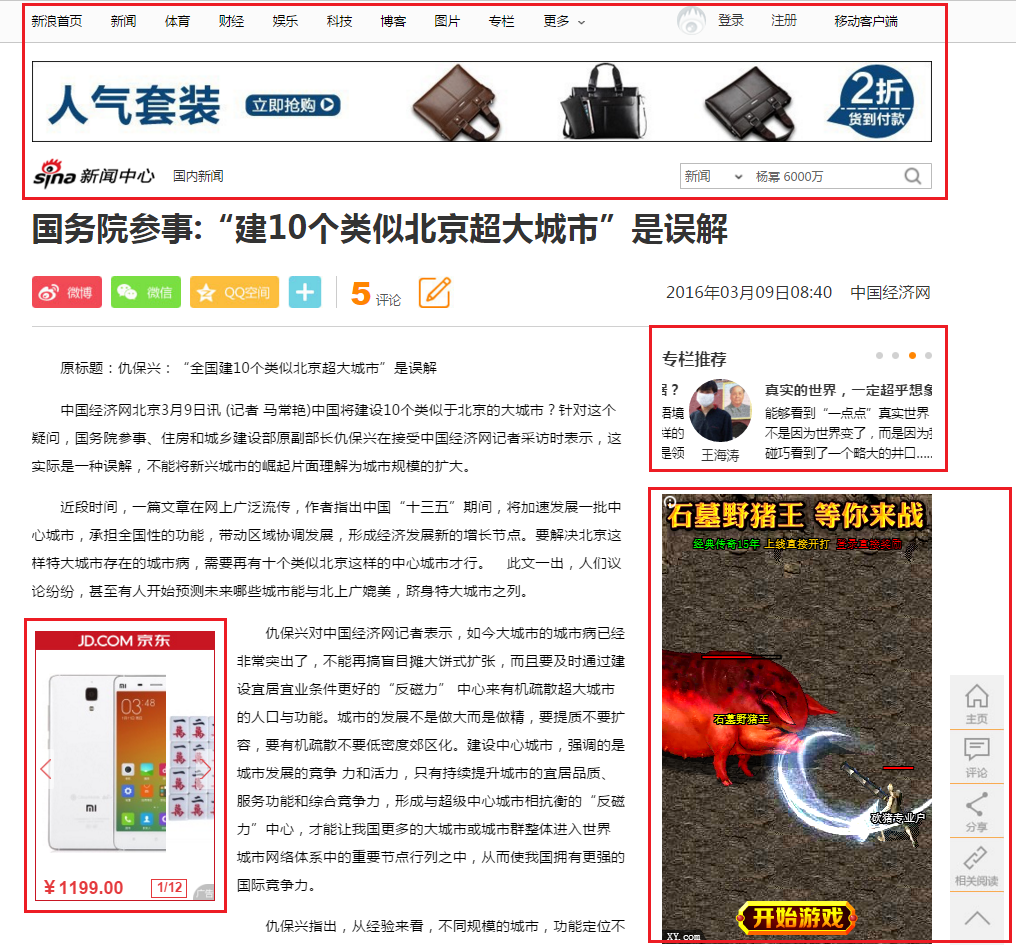
\includegraphics[width=0.9\textwidth,height=0.45\textheight]{news}
\caption{新浪新闻实例}
\label{fig:news}
\end{figure}

\begin{figure}[htbp]
\centering
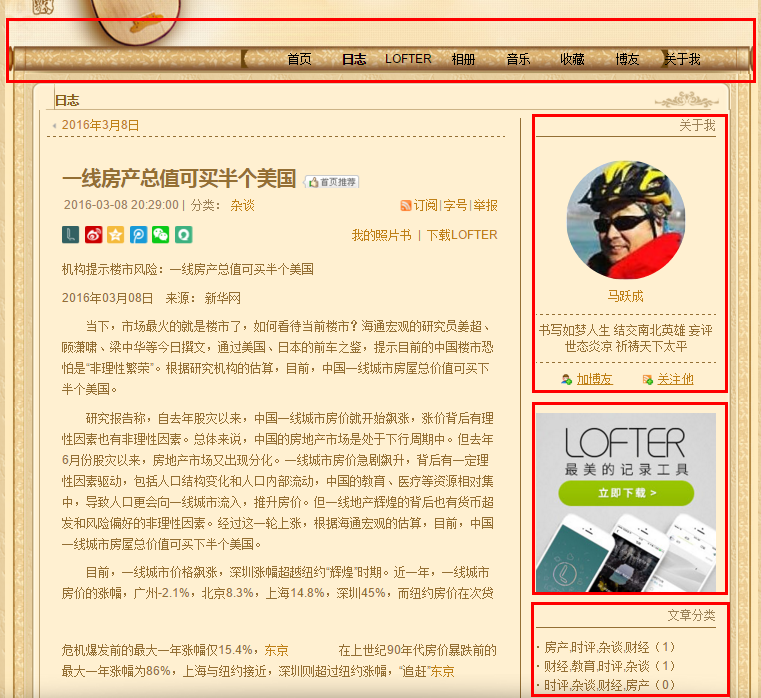
\includegraphics[width=0.9\textwidth,height=0.45\textheight]{blog}
\caption{网易博客实例}
\label{fig:blog}
\end{figure}

从新闻、博客网页中抽取核心内容,过滤这些噪声,不仅能够给用户提供“干净”的内容,
也能节约爬虫系统的存储开销,减小索引规模,提升后续自然语言处理的效果。
研究模板无关的自动化内容抽取技术,对爬虫系统的可扩展性和易维护性具有重要意义。

由于新闻和博客网页布局与内容抽取目标的相似性,本章将两者合并处理,
提出一种基于有效字符的Web内容抽取方法。
~\ref{sec:cevc-other}~节简单介绍对比算法CETR(基于文本标签比)、CETD(基于文本密度)
和CEPR(基于文本标签路径比)的原理及实现细节;
~\ref{sec:cevc-method}~节详述本文提出的基于有效字符的Web内容抽取算法CEVC
(Content Extraction via Valid Characters);
~\ref{sec:cevc-experiment}~节进行新闻和论坛的内容抽取实验,并分析实验结果;
~\ref{sec:cevc-conclusion}~节总结本章。

\section{对比算法及实现}
\label{sec:cevc-other}

\subsection{基于文本标签比的内容抽取算法}
Weninger等人于2010年提出
基于文本标签比的内容抽取算法CETR(Content Extraction via Tag Ratios)
\citeup{weninger2010cetr}。

CETR的基本概念是定义了Tag Ratio。
它以“行”为单位读取HTML网页并处理,分别计算每一行的Tag Ratio,
即非HTML标签字符个数与HTML标签个数的比值。
如果遇到HTML标签个数为零的特殊情况,该行的Tag Ratio就是所有字符的个数。
作者认为Tag Ratio越高,反映了文本密集程度越高,更有可能是网页的核心内容。

通过计算可以得到每一行Tag Ratio的直方图,最直接的方法就是找到一个阈值,
所有Tag Ratio高于此阈值的行被认为是有效内容,
所有Tag Ratio低于此阈值的行被认为是噪声内容。
如何找到这样一个合适的阈值,就成为了文章的主要研究内容。

为了提升直方图的区分度,作者对数据进行了高斯平滑。
标准的高斯平滑算法主要用来做图像处理,是应对连续数据的,作者重新实现为一维的离散操作。
公式(~\ref{eq:cetr-kernel}~)是高斯核函数的构造过程,
给定窗口大小为$2(\lceil \sigma \rceil) + 1$。

\begin{equation}
\label{eq:cetr-kernel}
k_i = \sum_{j=-\lceil \sigma \rceil}^{\lceil \sigma \rceil}
e^{\frac{-j^2}{2\sigma^2}}, 0 \leq i \leq 2(\lceil \sigma \rceil)
\end{equation}

公式(~\ref{eq:cetr-kernel2}~)中高斯核函数$k$被处理为$k'$。

\begin{equation}
\label{eq:cetr-kernel2}
k_i' = \frac{k_i}{\sum_{j=0}^{\lceil \sigma \rceil}k_j},
\lceil \sigma \rceil \leq i \leq 2(\lceil \sigma \rceil)
\end{equation}

最后高斯核函数$k'$和直方图$T$一起做卷积运算,形成平滑后的直方图$T'$,
如公式(~\ref{eq:cetr-kernel3}~)所示。

\begin{equation}
\label{eq:cetr-kernel3}
T_i' = \sum_{j=-\lceil \sigma \rceil}^{\lceil \sigma \rceil}
k'_{j+\lceil \sigma \rceil} T_{i-j},
\lceil \sigma \rceil \leq i \leq len(T)-\lceil \sigma \rceil
\end{equation}

上述以阈值划分直方图的方法,其缺陷是将Tag Ratio仅仅视为一组数据,
而不是有序的序列,为了利用有序的信息,作者提出了一个二维模型。

\begin{equation}
\label{eq:cetr-kernel4}
f'(T_i')=G_i=\frac{\sum_{j=0}^{\alpha} T_{i+j}'}{\alpha} - T_i',
0 \leq i < len(T') - \alpha
\end{equation}

注意到$len(G) \neq len(T')$,实际上$len(G)=len(T')-1$
因为$G$是一组数据的差异值。
接着使用公式(~\ref{eq:cetr-kernel3}~)平滑$G$得到$G'$。
最后计算$\hat{G}$使得$\hat{G_i}=\vert G_i' \vert$,对于$G'$中的每一个$i$。

将平滑后的Tag Ratio $T'$和$T'$的Absolute Smoothed Derivatives $\hat{G}$
联合组成二维模型,相比于一维数据,更加具有区分度。

随后作者使用K-means聚类算法,将所有的样本点进行聚类,这里使用$k=3$。
与一般的K-means聚类不同,将其中一个簇的中心点固定为二维坐标系的原点,
这样可以使得剩余簇远离原点,并且很容易划分最终的结果,
即中心点固定在原点的簇是噪声内容,而剩余簇代表有效内容。

作者一共提出了三种算法,记为CETR-TM、CETR-KM和CETR。
CETR-TM是阈值算法,CETR-KM是一维数据上的K-means聚类算法,
CETR是二维数据上的K-means聚类算法。
根据作者的实验对比,CETR的抽取性能最佳,也是本章中参与对比的算法。

作者提供了Java实现的算法源代码\footnote{http://www3.nd.edu/~tweninge/cetr/},
我们对其进行了简单的包装,以Python接口调用并参与后续的评价指标计算。

\subsection{基于文本密度的内容抽取算法}
Sun等人于2011年提出
基于文本密度的内容抽取算法CETD(Content Extraction via Text Density)
\citeup{sun2011dom}。

CETD算法的核心概念是Text Density,它在DOM树的基础上定义,
而不像CETR那样以行为单位处理,更能利用HTML的结构信息。
Text Density的基础定义如~\ref{def:cetd-td}~所示。

\begin{definition}
\label{def:cetd-td}
如果$i$是一个标签(对应DOM树中的一个节点),那么$i$的Text Density($TD_i$)
是其字符个数和标签个数的比值:
\begin{equation}
TD_i = \frac{C_i}{T_i}
\end{equation}
\end{definition}

在进一步研究后,作者发现很多网页噪声由超链接组成,基于这样的观察,
对每个节点计算了两个额外的统计指标:
\begin{enumerate}
\item \textit{LinkCharNumber}:子树中所有链接字符的个数
\item \textit{LinkTagNumber}:子树中所有链接标签的个数
\end{enumerate}

在加入了链接的统计信息后,定义了Composite Text Density:

\begin{definition}
\label{def:cetd-ctd}
如果$i$是一个标签(对应DOM树中的一个节点),
那么$i$的Composite Text Density($CTD_i$)是:
\begin{equation}
CTD_i = \frac{C_i}{T_i}\log_{ln(\frac{C_i}{\neg LC_i}LC_i + 
\frac{LC_b}{C_b}C_i + e)}(\frac{C_i}{LC_i}\frac{T_i}{LT_i})
\end{equation}
\end{definition}

定义~\ref{def:cetd-ctd}~中,$C_i$表示$i$节点下的所有字符个数,
$T_i$表示$i$节点下的所有标签个数,$LC_i$表示链接字符个数,
$\neg LC_i$表示非链接字符个数,$LT_i$表示链接标签个数,
$LC_b$表示\texttt{<body>}节点下的所有链接字符个数,
$C_b$表示\texttt{<body>}节点下的所有字符个数。
遇到分母为零的情况,直接将分母设为1。

为了从Text Density中区分噪音节点和内容节点,
最直接的方法是以\texttt{<body>}的Text Density作为划分阈值。
因为\texttt{<body>}比噪音节点包含更多的文本内容,
又比内容节点包含更多的超链接,所以它是一个足够区分二者的中间值。

数据平滑可以削峰填谷,增加区域内部的内聚性和区域之间的差异性,
虽然一般来说数据平滑可以取得较好的结果,它仍然会丢失一些低文本密度的节点。
为了改进传统的平滑、基于阈值划分的方法,作者提出了DensitySum的方法。

DensitySum基于这样的观察,网页的内容块在DOM树结构中都属于一个祖先节点,
并且内容节点的文本密度显著高于噪声节点。
如果把一个节点的所有子节点的文本密度累加,称为DensitySum,
那么DensitySum就会在内容节点上取得一个极高值。
其定义如下:

\begin{definition}
\label{def:cetd-densitysum}
如果$N$是一个标签(对应DOM树中的一个节点),$i$是$N$的一个子节点,
那么$N$的DensitySum就是它所有子节点文本密度之和:
\begin{equation}
DensitySum_N = \sum_{i \in C} TextDensity_i
\end{equation}
\end{definition}

作者一共提出了三种算法CETD-DS,CECTD-S和CECTD-DS。
CETD-DS是基于Text Density和DensitySum的算法,
CECTD-S是基于Composite Text Density和数据平滑的算法,
CECTD-DS是基于Composite Text Density和DensitySum的算法。
根据作者的实验对比,CECTD-DS的抽取性能最佳,也是本章中参与对比的算法。
如无特殊说明,以后简称CECTD-DS为CETD算法。

根据文献\cite{sun2011dom}给出的算法伪代码,我们用Python 2.7重新实现了CETD。
为了处理HTML文档中的错误,同样使用了BeautifulSoup尽可能纠正。
并通过BeautifulSoup,将HTML文档转化为内存中的DOM树,
在进行计算和操作之前去除了所有\texttt{<script>},\texttt{<style>}和\texttt{comment}。

\subsection{基于文本标签路径比的内容抽取算法}
Wu等人于2013年提出了
基于文本标签路径比的内容抽取算法CEPR(Content Extraction via Path Ratios)
\citeup{wu2013web}。

CEPR算法的核心概念是\textbf{T}ext to Tag \textbf{P}ath \textbf{R}atio,或简称为TPR。
作者首先在DOM树的基础上,提出Tag Path的概念,
即从根节点到文本叶节点\footnote{文本全部分布在DOM树的叶节点上,见~\ref{subsec:dom}~节}
的一条路径,由HTML标签构成。
例如\texttt{div.div.div.h1}就是一条Tag Path。
在Tag Path的基础上,提出Text to Tag Path Ratio:

\begin{definition}
\label{def:cepr-tpr}
假设$p$是一条Tag Path,那么$p$的Text to Tag Path Ratio(TPR)就是:
\begin{equation}
TPR(p) = \frac{\sum_{v \in accNodes(p)}length(c(v))}{\vert accNodes(p) \vert}
\end{equation}
\end{definition}

定义~\ref{def:cepr-tpr}~中,$accNodes(p)$是路径$p$能够访问的文本叶节点集合,
$c(v)$是文本叶节点$v$的文本内容。
TPR既是每条Tag Path的度量值,也是每个文本叶节点的度量值。
在一般网页上,通常有这样的观察:
\begin{enumerate}
\item 内容节点通常有相似的Tag Path,而噪声节点也有相似的Tag Path;
\item 内容节点通常包含更多的文本,而噪声节点通常包含较少的文本;
\item 所有文本节点都是叶节点。
\end{enumerate}
显然,内容节点的TPR值较高而噪声节点的TPR值较低,可以用来抽取核心内容。
TPR的阈值定为$\tau = \lambda \sigma(H')$,$\lambda$是调节参数,
$\sigma(H')$是直方图的标准差。

进一步的研究表明,网页内容会包含标点符号,而噪声则没有。
除此之外,文本长度和标点符号个数在内容节点中的分布差异很大,在噪声节点中却很少变化。
作者进一步提出了
\textbf{E}xtended \textbf{T}ext to Tag \textbf{P}ath \textbf{R}atio(ETPR):

\begin{definition}
\label{def:cepr-etpr}
假设$p$是一条Tag Path,那么$p$的Extended Text to Tag Path Ratio(ETPR)就是:
\begin{equation}
ETPR(p) = TPR(p) \cdot 
\frac{\sum_{v \in accNodes(p)}puncNum(c(v))}{\vert accNodes(p) \vert}
\cdot \sigma_{cs} \cdot \sigma_{ps}
\end{equation}
\end{definition}

定义~\ref{def:cepr-etpr}~中$puncNum(c(v))$是$v$中标点符号的个数,
$\sigma_cs$和$\sigma_ps$分别是路径$p$能访问的文本叶节点集合中
文本长度和标点符号个数的标准差。

在文献\cite{weninger2010cetr}的高斯平滑算法基础上,
作者提出以编辑距离作为权重,改善平滑效果。
即公式(~\ref{eq:cetr-kernel3}~)的卷积运算修改为公式(~\ref{eq:cepr-kernel}~)。

\begin{equation}
\label{eq:cepr-kernel}
H_i' = \sum_{j=-r}^{r} w_{ij} k_j' H_{i-j}, r \leq i \leq len(H)-r
\end{equation}

其中权重定义为:
\begin{equation}
\label{eq:cepr-w}
w_{ij} = 
\left\{\begin{matrix}
1, p_i = p_j \\ 
\frac{1}{(dist(p_i, p_j))^\alpha}, p_i \neq p_j
\end{matrix}\right.
\end{equation}

公式(~\ref{eq:cepr-w}~)中的$dist(p_i, p_j)$是路径$p_i$和$p_j$的
编辑距离\citeup{levenshtein1966binary},
$\alpha$是调节编辑距离对平滑贡献的参数。

作者一共提出了三种算法CEPR-TPR,CEPR-ETRP和CEPR-SETPR。
CEPR-TPR是基于TPR的算法,CEPR-ETPR是基于扩展的ETPR的算法,
CEPR-SETPR是基于ETPR并进行加权高斯平滑处理后的算法。
根据作者的实验对比,CEPR-SETPR的抽取性能最佳,也是本章中参与对比的算法。
如无特殊说明,以后简称CEPR-SETPR为CEPR算法。

根据文献\cite{wu2013web}给出的算法伪代码,我们用Python 2.7重新实现了CEPR。
同样使用了BeautifulSoup来处理HTML文档,转化为DOM树结构。
CEPR算法需要判断标点符号,这里使用了Python标准库的\texttt{string.punctuation}
来定义英文标点符号,并补充了一个中文标点符号列表。
CEPR算法需要计算路径的编辑距离,这里以Tag的尺度计算,
而不是直接计算两个Tag Path字符串的编辑距离。

我们在小规模数据集上进行了参数调整实验,确定了和文献\cite{wu2013web}中一致的参数配置:
$\lambda=0.8$,$\alpha=1$和$r=1$。

\section{基于有效字符的Web内容抽取算法}
\label{sec:cevc-method}

\subsection{文档对象模型(DOM)}
\label{subsec:dom}
在网页内容抽取的研究工作中,为了利用HTML文档的结构信息,
很多方法都是在DOM的基础上进行\citeup{yi2003eliminating,sun2011dom,wu2013web}
这里对DOM做简单介绍。

DOM(Document Object Model,文档对象模型)是一个跨平台语言无关的规范,
用来表示和操作HTML,XHTML和XML的对象\footnote{http://www.w3.org/DOM/}。
每个文档所包含的节点被组织为一个树型结构,称为DOM树。
DOM树节点所表示的对象可以通过一组方法来寻址或操作,这些接口以API的形式描述。
通过这样一种规范,程序和脚本能够动态访问和更新文档的内容、结构以及风格,
文档经过后续处理后,还能将结果更新到展示的页面上。

上世纪90年代,网景公司和微软公司相继推出自己的浏览器,和浏览器端的脚本语言JavaScript。
JavaScript让Web开发者能够创造和用户交互的网页,检测用户产生的事件并更新HTML文档,
这类第一代的语言被称为Legacy DOM。
随后W3C(World Wide Web Consortium,万维网联盟)制定了第一版的DOM标准,
之后相继发布了新版本。
截止到2005年,W3C DOM中的大部分特性都能被主流浏览器广泛支持。

HTML文档可以解析为DOM树,每个HTML标签对应一个DOM树节点,
父子节点对应HTML标签的嵌套关系,兄弟节点对应HTML标签的并列关系,
这样就把序列化的HTML文档转换为层次化的对象模型,便于程序的访问和操作。

\begin{example}
\label{ex:html}
一个简化的HTML代码片段
\end{example}
\begin{oframed}
\begin{verbatim}
 1. <html>
 2.   <head> ... </head>
 3.   <body>
 4.     <div class="nav-wrap">
 5.       <h1>Small Vintage Plane Crashes in Hudson River</h1>
 6.     </div>
 7.     <div> ... </div>
 8.     <div class="ep-content">
 9.       <a>
10.         <span>From Stefan Holt</span>
11.       </a>
12.       <p>The plane was on a photo flight with two other planes...</p>
13.       <p>They say they saw the pilot try to get out but...</p>
14.     </div>
15.   </body>
16. </html>
\end{verbatim}
\end{oframed}

\begin{figure}[htbp]
\centering
\begin{tikzpicture}[
sibling distance=4cm,
tag/.style={circle, draw},
leaf/.style={rectangle, draw, text width=3.5cm}
]
\node[tag]{html}
  child{node[tag]{head}}
  child{node[tag]{body}
    child{node[tag]{div}
      child{node[tag]{h1}
        child{node[leaf]{\footnotesize Small Vintage Plane Crashes in Hudson River}}
      }
    }
    child{node[tag]{div}}
    child{node[tag]{div}
      child{node[tag]{a}
        child{node[tag]{span}
          child{node[leaf]{\footnotesize From Stefan Holt}}
        }
      }
      child{node[tag]{p}
        child{node[leaf]{\footnotesize The plane was on a photo flight with two other planes}}
      }
      child{node[tag]{p}
        child{node[leaf]{\footnotesize They say they saw the pilot try to get out but}}
      }
    }
  }
;
\end{tikzpicture}
\caption{一个简化的DOM树}
\label{fig:dom}
\end{figure}

例~\ref{ex:html}~所示的HTML片段经过解析后形成一个DOM树,如图~\ref{fig:dom}~所示。
每个HTML标签都与一个DOM树节点对应,HTML标签的属性仍然附属在DOM节点上。
网页中能够显示的具体文本都位于DOM树的叶节点上,DOM树的内部节点只负责结构控制和布局。
HTML的根节点是\texttt{<html>},一般包含两个节点\texttt{<head>}和\texttt{<body>}。
网页的可视区域都从\texttt{<body>}标签开始,
因此我们的研究对象是\texttt{<body>}标签下的内容。

\subsection{有效字符定义与统计方法}
回顾图~\ref{fig:news}~和~\ref{fig:blog}~,我们注意到网页正文一般是文本密集的区域,
而噪声信息则包含高度格式化的、简短的文本。
通过大量实例分析,我们发现噪声信息通常包含链接,无论是导航栏的网站板块链接,
还是广告链接或相关文章链接,它们都符合这个特点,吸引用户点击来完成自己的职能。
反之,一段不包含链接的文本更有可能是网页核心内容。

链接在HTML文档中由\texttt{<a>}标签组成,a代表anchor,所以链接内的文本也称为锚文本。
DOM节点的继承关系使得包裹在\texttt{<a>}标签内的所有文本都变成锚文本,
例如图~\ref{fig:dom}~中的\texttt{From WWW}虽然在\texttt{<span>}下,
但其祖先节点是一个\texttt{<a>}标签,因此也变成了锚文本。

除此之外,噪声信息较为简短,甚至不能组成一个语义完整的句子,我们可以利用停止词来刻画这一特征。
停止词是自然语言处理中过滤掉的词\footnote{https://en.wikipedia.org/wiki/Stop\_words},
它们在一篇文章中大量出现,多为冠词、介词或连词,却对文章主体内容贡献很小。
尽管停止词对文章没有多大意义,但一段话如果没有停止词,那么它就不是一个语义完整的句子,
更有可能是一组关键词的堆砌,而不是网页的核心内容。
例~\ref{ex:stopwords}~节选自网页中的一段话,
以\underline{下划线}的形式标注了其中的停止词,
可见停止词在正文中是普遍存在的。

\begin{example}
\label{ex:stopwords}
网页中的停止词示例
\end{example}
\begin{oframed}
买房\underline{还是}租房?
\underline{这是}眼下很多\underline{人}要面对\underline{的}一道选择题。
如果简单比较,一边\underline{是}数额很大\underline{的}买房负担,
一边\underline{是}相对\underline{可}接受\underline{的}租金价格,
似乎租房应更受欢迎,现实\underline{却}非如此。
山东某县一位购房者对笔者道出心声:“买房子,政府一平方米补贴100元,一套房子能省1万多元。
租房子,\underline{啥}实惠没有,\underline{还}总\underline{被}赶来赶去,
住\underline{着不}踏实。”
\underline{他}最终\underline{还是}选择\underline{了}勒紧裤腰带贷款买房。
\end{oframed}

结合上述链接和停止词与网页噪声的相关性,我们提出一个有效字符的概念:

\begin{definition}
\label{def:validchar}
$i$是DOM中的一个叶节点,如果$\forall p \in ancestors(i)$都有$tag(p) \neq a$,
并且$stopwords(i) > 0$,那么$i$所包含的文本就是有效字符。
\end{definition}

定义~\ref{def:validchar}~中,$ancestors(i)$表示$i$的所有祖先节点,
$tag(p)$表示$p$的标签名,$stopwords(i)$表示$i$的停止词个数。
有效字符代表网页中那些更有可能是正文的文本,忽略了链接噪声和太过松散的短语,
有效字符越多,代表这个节点更有可能是正文。

为了利用DOM节点的有效字符分布信息,我们需要计算每个DOM节点下所包含的有效字符个数,
可以将其作为一项属性,插入到DOM节点中,便于后续的处理。
在计算之前,首先去除网页中的\texttt{<script>},\texttt{<style>}和\texttt{comment}。
这些脚本、样式文件和注释对网页显示的文本内容没有贡献,却可能干扰计算结果。

如算法~\ref{algo:cevc-count}~所示,这是一个自顶向下的递归计算过程。
ValidChars被作为属性,存储在节点中。
当前节点有子节点时,递归计算子节点,然后当前节点的有效字符数被累加到父节点上。
当前节点是叶节点时,根据定义~\ref{def:validchar}~判断它包含的文本是否是有效字符,
如果是,则将非空白字符数累加到父节点上。
这里忽略了空白字符,是为了排除网页排版风格带来的影响,让计算结果更加稳定。

算法~\ref{algo:cevc-count}~的主要操作就是遍历DOM树,
所以它的运行时间与DOM树中的节点数成正比,时间复杂度为$O(n)$,$n$是DOM树中的节点数。
为了在内存中存储解析后的DOM树,其空间复杂度也是$O(n)$。

\begin{algorithm}[htbp]
\caption{countValidChars(N)}
\label{algo:cevc-count}
\KwIn{DOM node N}
\KwOut{DOM node N}

\eIf{N has child nodes} {
  \For{C $\in$ N.children()}{
    countValidChars(C) \;
  }
  N.parent.validChars += N.validChars \;
}{
  \tcp{N is a leaf text node}
  \If{N consists of valid characters}{
    length = getNonSpaceLength(N) \;
    N.parent.validChars += length \;
  }
}
\end{algorithm}

经过算法~\ref{algo:cevc-count}~的处理,
我们可以得到一个标注了各个节点ValidChars的HTML页面,如图~\ref{fig:news-stepinto}~所示。

\begin{figure}[t]
\centering
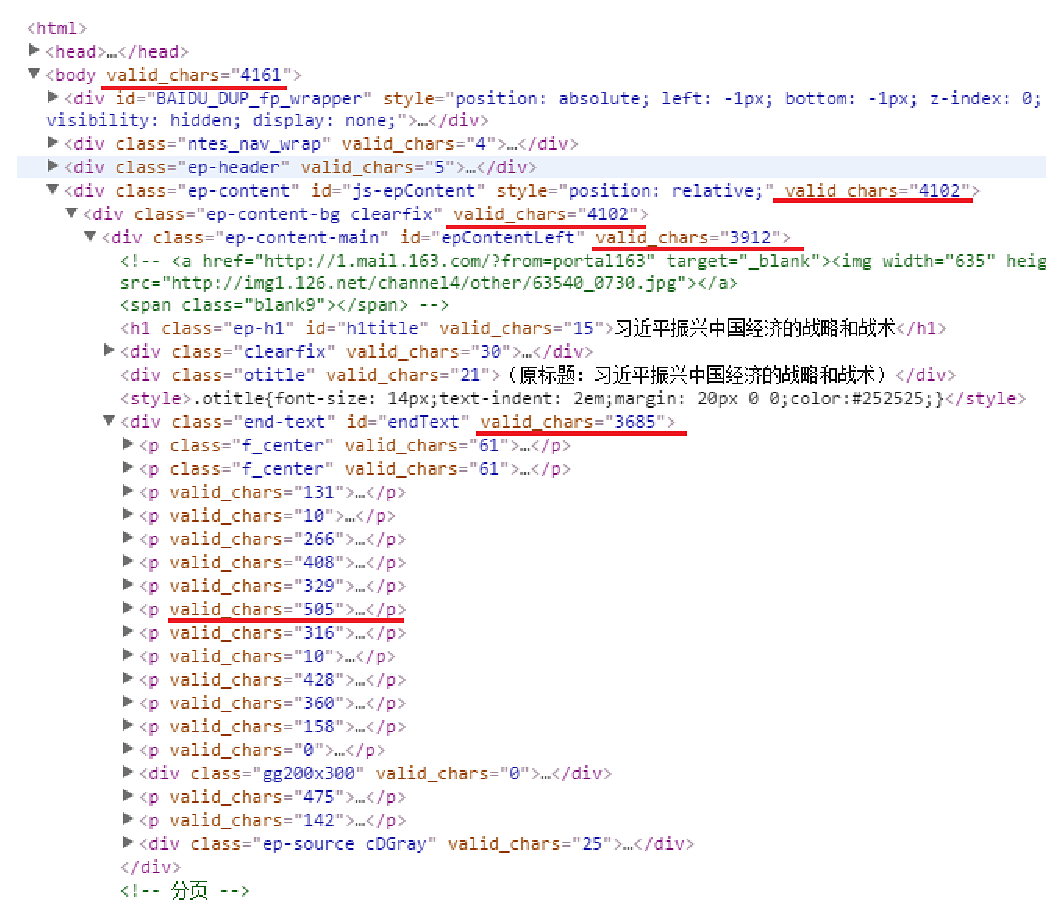
\includegraphics[width=0.9\textwidth]{news-stepinto}
\caption{有效字符示例}
\label{fig:news-stepinto}
\end{figure}

\subsection{核心内容块定位方法}
经过大量实例分析,我们发现对于新闻、博客这类正文信息集中的网站,
核心内容块都位于同一个父节点之下,通常表现为文本的段落。
图~\ref{fig:news-stepinto}~中的新闻正文位于\texttt{<div\#endText>}节点之下,
是由\texttt{<p>}标签构成的段落。

这里\texttt{div\#endText}的记号是CSS选择符,可以指定CSS样式规则作用在哪些DOM节点上,
简单的用法是\texttt{div\#endText}选择\texttt{<div id='endText'>}这样的标签,
而\texttt{div.text}选择\texttt{<div class='text'>}这样的标签。
和正则表达式、XPath一样,CSS选择符也可以用来在HTML文档中描述提取规则。

现在我们看到每个DOM节点上都标注了有效字符的个数,有效字符越多表明这个节点越可能是核心内容。
但这个比较必须在同一个层次的兄弟节点间才有意义,因为有效字符数是嵌套包含的,
毫无疑问\texttt{<body>}的有效字符数最多。
如果从\texttt{<body>}节点开始,每次都选择有效字符数最多的子节点深入,
就能定位出一条从\texttt{<body>}通往核心内容块的正确路径,
如图~\ref{fig:news-stepinto}~中红线标示的节点。

每次沿着有效字符数最大的子节点不断深入,意味着我们每一步放弃了信息量较小的兄弟节点。
这个过程不能一直持续下去,否则会陷入到叶节点中,而错失最终的父节点。
如图~\ref{fig:news-stepinto}~所示,最后一步进入了一个\texttt{<p>}标签,
而错失了真正的核心内容块\texttt{<div\#endText>}。
我们需要定义一个指标,来判断何时停止向下深入的过程。

\begin{definition}
\label{def:mcr}
$i$是DOM树中的一个节点,$i$的最大子节点字符占比MCR(Max Chars Ratio)如下所示,
其中$C_i$表示$i$的有效字符数,$j$是$i$的子节点:
\begin{equation}
MCR_i = max_{j \in children(i)} \frac{C_j}{C_i}
\end{equation}
\end{definition}

在DOM树中每次向下深入一步,我们认为最大子节点包含了父节点的绝大部分文本信息。
当定义~\ref{def:mcr}~中的MCR低于一个阈值时,
表明最大子节点的有效字符数并不足以在父节点中占据统治地位,
即最大子节点的文本不能在可接受的损失范围内代表父节点,这时候放弃兄弟节点是不合理的,
因此向下深入的过程应立即终止,当前节点就是核心内容块。

\begin{example}
\label{ex:mcr}
MCR计算过程
\end{example}
\begin{oframed}
\begin{verbatim}
1. <body> valid_chars=4161 MCR=0.99
2. <div#js-epContent> valid_chars=4102 MCR=1.0
3. <div.ep-content-bg> valid_chars=4102 MCR=0.95
4. <div#epContentLeft> valid_chars=3912 MCR=0.94
5. <div#endText> valid_chars=3685 MCR=0.14 核心内容块
6. <p> valid_chars=505
\end{verbatim}
\end{oframed}

如例~\ref{ex:mcr}~所示,每一行显示的都是图~\ref{fig:news-stepinto}~中各层的最大子节点。
在到达\texttt{<body\#endText>}之前,MCR一直保持$0.9$以上的高比率,
而\texttt{<body\#endText>}的MCR锐减到$0.14$,因为此时已深入到正文的一个段落中,
这个段落无法代表正文的内容,\texttt{<body\#endText>}就是最终的核心内容块。

上述过程如算法~\ref{algo:cevc-stepinto}~所示。
在经过算法~\ref{algo:cevc-stepinto}~\texttt{countValidChars}预处理后的DOM树上,
先遍历子节点,找出有效字符数最大的子节点,并累加所有字符数。
然后选定最大子节点\texttt{maxNode},如果MCR小于一个阈值$\alpha$就停止并输出当前节点,
否则在MaxNode上继续递归调用算法\texttt{stepInto}。
\texttt{output}过程负责把当前节点的所有有效字符输出,作为核心内容抽取的结果返回。
注意第~\ref{algo:line:edge}~行,当遇到一种极端情况,正文仅仅包含一个段落,
那么StepInto深入到最底层仍然会有很高的MCR,导致无法终止直到进入叶节点。
这时候采取一种简单的策略,认为当前节点的父节点就是核心内容块。
后续实验表明,这是一个简单也可以接受的方案。

通过在DOM树中不断选择最有代表性的子节点不断深入,
算法~\ref{algo:cevc-stepinto}~至多被递归调用$h$次,
$h$是DOM树的高度,所以其时间复杂度为$O(h)$,能够很快运行结束。

\begin{algorithm}[htbp]
\caption{stepInto(N)}
\label{algo:cevc-stepinto}
\KwIn{DOM node N}
\KwOut{main content}

maxNode = null \;
maxValidChars = 0 \;
totalValidChars = 0 \;
\For{$C \in N.children()$}{
  totalValidChars += C.validChars \;
  \If{$C.validChars > maxValidChars$}{
    maxValidChars = C.validChars \;
    maxNode = C \;
  }
}

\eIf{maxNode is not null}{
  MCR = maxValidChars / totalValidChars \;
  \eIf{$MCR < \alpha$}{
    \Return output(N) \;
  }{
    stepInto(maxNode) \;
  }
}{
  \tcp{Step into the leaf node}
  \Return output(N.parent) \; \label{algo:line:edge}
}
\end{algorithm}

\subsection{算法实现概述}
面对HTML网页中普遍存在的代码错误,例如缺失结束标签、使用非标准的标签和错误的嵌套等,
这里使用Python第三方库
BeautifulSoup\footnote{http://www.crummy.com/software/BeautifulSoup/}
来尽可能纠正这些错误。
BeautifulSoup是一个可以从HTML或XML文件中提取数据的Python库,
它为操作DOM提供了一套方便的接口,底层调用lxml等具体的解析器,
能够处理有代码错误的网页。

CEVC算法中需要识别停止词,这里使用了
jieba\footnote{https://github.com/fxsjy/jieba}中的停止词模块。
jieba(结巴中文分词)是一个开源的Python中文分词组件,MIT协议授权,
支持多种分词模式。

\section{新闻和博客的内容抽取实验}
\label{sec:cevc-experiment}

\subsection{内容抽取评价指标}
为了验证算法的抽取效果,我们定义标准评价指标精确率Precision、召回率Recall和
F\textsubscript{1}。
通过比较算法抽取的文本$e$和金标准的文本$g$,Precision、Recall和
F\textsubscript{1}可以如下计算:

\begin{equation}
P = \frac{LCS(e,g).length}{e.length}, R = \frac{LCS(e,g).length}{g.length}
\end{equation}
\begin{equation}
F_1 = \frac{2 \times P \times R}{P + R}
\end{equation}

对于中文文档,视为字符的序列而不进行分词处理,
因为中文分词需要额外的依赖,而且CEVC算法重在对有效字符的统计而不需要词的信息。
$LCS(e,g)$是$e$和$g$的最长公共子序列,
文档中两个相同的字符如果位置顺序不同,也会被LCS的计算区分开来。
相比于文献\cite{weninger2010cetr}中使用的计算方法,把两个文档的词视为两个集合,
该方法利用了不同词的位置信息而更加准确。

在计算一个网站或一个算法整体的评价指标时,是将每个单独网页的最长公共子序列长度累加计算的,
而不是简单计算平均值,Precision如下所示,Recall和F\textsubscript{1}的计算类似。

\begin{equation}
P = \frac{\sum LCS(e_i,g_i).length}{\sum e_i.length}
\end{equation}

除了标准评价指标外,这里给出另一个常用的评价方法Score。
Score在文献\cite{sun2011dom}和文献\cite{wu2013web}中都提到过,
是为了替换CleanEval中运算开销很大的
Levenshtein Distance\citeup{levenshtein1966binary}
(对齐两个字符串所需要的插入、删除操作次数,不允许替换),
而使用最长公共子序列计算产生的。
其定义如下:

\begin{equation}
Score(e,g) = \frac{LCS(e,g).length}{e.length + g.length - LCS(e,g).length}
= \frac{1}{\frac{1}{P} + \frac{1}{R} - 1}
\end{equation}

\subsection{新闻和博客数据集}

为了在验证内容抽取算法对当今中文新闻、博客网站的实际抽取效果,
我们从知名的网址导航网站hao123\footnote{https://www.hao123.com/}
和360导航\footnote{https://hao.360.cn/}
中任意选取了30个知名的新闻网站和博客网站作为测试对象。
网站详情和网页数量见表~\ref{tbl:news-dataset}~和表~\ref{tbl:blog-dataset}~。

对每个网站,我们分别编写爬虫脚本下载原始HTML网页,
然后通过人工编写的包装器抽取网页正文作为金标准,并存储为UTF-8编码的文本文件。
为了确保数据集的质量,还对包装器抽取的文本进行了人工审核,
排除了抽取错误的网页和正文不足100字的网页。
15个新闻网站和15个博客网站总计含有1270个有效网页。

\begin{table}[htbp]
\centering
\begin{minipage}{0.45\textwidth}
\caption{新闻数据集}
\label{tbl:news-dataset}
\vspace{0.5em}\centering\wuhao
\begin{tabular}{lll}
\toprule[1.5pt]
网站 & 网址 & 数量 \\
\midrule[1pt]
网易新闻 & news.163.com & 47 \\
央视网新闻 & news.cctv.com & 45 \\
凤凰资讯 & news.ifeng.com & 47 \\
腾讯新闻 & news.qq.com & 53 \\
新浪新闻 & news.sina.com.cn & 39 \\
搜狐新闻 & news.sohu.com & 34 \\
中国军网 & www.81.cn & 48 \\
参考消息 & www.cankaoxiaoxi.com & 40 \\
中国信息网 & www.chinanews.com & 46 \\
央广网 & www.cnr.cn & 44 \\
环球网 & www.huanqiu.com & 43 \\
人民网 & www.people.com.cn & 39 \\
南方网 & www.southcn.com & 50 \\
新华网 & www.xinhuanet.com & 39 \\
联合早报 & www.zaobao.com & 36 \\
总计 & - & 650 \\
\bottomrule[1.5pt]
\end{tabular}
\end{minipage}
\hfill
\begin{minipage}{0.45\textwidth}
\caption{博客数据集}
\label{tbl:blog-dataset}
\vspace{0.5em}\centering\wuhao
\begin{tabular}{lll}
\toprule[1.5pt]
网站 & 网址 & 数量 \\
\midrule[1pt]
网易博客 & blog.163.com & 48 \\
财经网博客 & blog.caijing.com.cn & 45 \\
中金博客 & blog.cnfol.com & 31 \\
东方财富博客 & blog.eastmoney.com & 46 \\
和讯博客 & blog.hexun.com & 45 \\
凤凰博客 & blog.ifeng.com & 45 \\
瑞丽博客 & blog.rayli.com.cn & 39 \\
科学网博客 & blog.sciencenet.cn & 47 \\
新浪博客 & blog.sina.com.cn & 42 \\
搜狐博客 & blog.sohu.com & 29 \\
天涯博客 & blog.tianya.cn & 50 \\
博客大巴 & www.blogbus.com & 13 \\
博客中国 & www.blogchina.com & 45 \\
博客网 & www.bokee.com & 46 \\
博客日报 & www.bokerb.com & 49 \\
总计 & - & 620 \\
\bottomrule[1.5pt]
\end{tabular}
\end{minipage}
\end{table}

\subsection{算法的参数调整}
CEVC算法中包含一个阈值参数$\alpha$,
它决定了什么时候终止算法~\ref{algo:cevc-stepinto}~中的向下深入过程。
$\alpha$的取值从0到1,如果它太低的话,终止条件就会很苛刻,
算法会因过于深入DOM树底层而返回一小段正文中的文本。
这种情况下因为损失了其它核心内容,召回率会下降。
另一方面,如果为$\alpha$设定一个过高的值,算法过早终止,
会返回不相关的内容,从而影响最终的精确率。

为了试验抽取性能和参数$\alpha$的关系,我们从各个网站中抽取少量网页进行了测试,
具体结果如图~\ref{fig:cevc-threshold}~所示。
召回率随着$\alpha$的升高而升高,精确率随着$\alpha$的升高而降低,总体趋势符合之前的期望。
从图中可以看到,作为一个综合性指标,
F\textsubscript{1}在$\alpha$从0.3增长到0.6的过程中都很稳定,保持在0.95以上。
CEVC算法对参数的变化并不敏感,因此在后续的实验中,设置$\alpha$为0.5。

\begin{figure}[htbp]
\centering
\begin{tikzpicture}
\begin{axis}[xlabel=$\alpha$, ylabel=Score (\%), legend pos=south east]
\addplot[color=blue, mark=square]
coordinates{
  (0, 99.3)(0.1, 99.4)(0.2, 99.4)(0.3, 99.5)(0.4, 99.5)(0.5, 99.5)
  (0.6, 99.5)(0.7, 97.5)(0.8, 97.3)(0.9, 95.0)(1.0, 88.8)
};

\addplot[color=blue, mark=triangle]
coordinates{
  (0, 61.9)(0.1, 79.0)(0.2, 92.3)(0.3, 96.7)(0.4, 96.7)(0.5, 96.7)
  (0.6, 96.7)(0.7, 96.7)(0.8, 96.7)(0.9, 96.7)(1.0, 96.9)
};

\addplot[color=blue, mark=star]
coordinates{
  (0, 76.2)(0.1, 88.0)(0.2, 95.8)(0.3, 98.1)(0.4, 98.1)(0.5, 98.1)
  (0.6, 98.1)(0.7, 97.1)(0.8, 97.0)(0.9, 95.9)(1.0, 92.7)
};

\legend{Precision, Recall, F\textsubscript{1}}
\end{axis}
\end{tikzpicture}
\caption{Precision, Recall和F\textsubscript{1}
随参数$\alpha$的变化情况}
\label{fig:cevc-threshold}
\end{figure}

\subsection{实验过程与结果}

实验环境为一台MacBook Pro(2 GHz Intel Core i7处理器,8G内存,256G SSD),
详细的实验过程如下:
\begin{enumerate}
\item 将下载的新闻、博客原始HTML网页以“网站名-URL的MD5.html”的形式命名,
包装器抽取并人工纠错的网页正文以UTF-8格式另存为“网站名-URL的MD5.txt”。
\item CETR、CETD、CEPR和CEVC四种算法分别用Python实现,并提供统一的调用接口,
输入HTML源文件,返回抽取的正文内容。
\item 编写测试脚本,分别调用不同的Web内容抽取算法,对测试数据集中的HTML网页抽取正文,
然后与金标准文本进行最长公共子序列计算,计算过程中字符串都是Unicode格式,确保编码一致。
\item 在计算一个网站或一个算法整体的评价指标时,
是将每个单独网页的最长公共子序列长度累加计算的,而不是简单计算平均值。
\item 实验结果以日志的形式保存在文件中,便于后续整理。
\end{enumerate}

首先对CEVC算法的抽取性能进行实验评估,
表~\ref{tbl:cevc-cevc}~给出了CEVC在新闻和博客数据集上的实验结果,
包含了Precision、Recall、F\textsubscript{1}和Score四项指标。

我们可以看到CEVC算法在30个不同的新闻、博客网站上都取得了良好的内容抽取效果。
对新闻网站的总体抽取效果达到了97.4\%的F\textsubscript{1},
对博客网站的总体抽取效果达到了94.4\%的F\textsubscript{1},
在所有测试集上,F\textsubscript{1}达到了95.8\%。
表明CEVC算法能够适应新闻、博客类网站的核心内容抽取需求。

\begin{table}[htbp]
\caption{CEVC在新闻和博客数据集上的实验结果}
\label{tbl:cevc-cevc}
\vspace{0.5em}\centering\wuhao
\begin{tabular}{lllllll}
\toprule[1.5pt]
网站 & 网址 & 类型 & Precision & Recall & F\textsubscript{1} & Score \\
\midrule[1pt]
环球网 & www.huanqiu.com & news & 91.1\% & 96.4\% & 93.7\% & 88.1\% \\
人民网 & www.people.com.cn & news & 96.2\% & 99.0\% & 97.6\% & 95.3\% \\
凤凰资讯 & news.ifeng.com & news & 99.5\% & 99.9\% & 99.7\% & 99.4\% \\
央视网新闻 & news.cctv.com & news & 93.7\% & 99.9\% & 96.7\% & 93.7\% \\
联合早报 & www.zaobao.com & news & 97.5\% & 99.1\% & 98.3\% & 96.7\% \\
新华网 & www.xinhuanet.com & news & 98.6\% & 99.9\% & 99.2\% & 98.5\% \\
中国信息网 & www.chinanews.com & news & 98.1\% & 99.9\% & 99.0\% & 98.0\% \\
中国军网 & www.81.cn & news & 97.6\% & 100.0\% & 98.8\% & 97.6\% \\
网易新闻 & news.163.com & news & 94.7\% & 98.8\% & 96.7\% & 93.7\% \\
腾讯新闻 & news.qq.com & news & 93.5\% & 99.9\% & 96.6\% & 93.4\% \\
央广网 & www.cnr.cn & news & 97.7\% & 99.5\% & 98.6\% & 97.2\% \\
参考消息 & www.cankaoxiaoxi.com & news & 95.3\% & 95.4\% & 95.3\% & 91.1\% \\
搜狐新闻 & news.sohu.com & news & 97.5\% & 97.8\% & 97.6\% & 95.4\% \\
南方网 & www.southcn.com & news & 91.5\% & 99.3\% & 95.2\% & 90.9\% \\
新浪新闻 & news.sina.com.cn & news & 96.3\% & 100.0\% & 98.1\% & 96.3\% \\
新闻 & - & - & 95.8\% & 99.1\% & 97.4\% & 95.0\% \\
\hline
和讯博客 & blog.hexun.com & blog & 96.4\% & 97.3\% & 96.8\% & 93.9\% \\
瑞丽博客 & blog.rayli.com.cn & blog & 86.6\% & 97.1\% & 91.6\% & 84.5\% \\
凤凰博客 & blog.ifeng.com & blog & 96.9\% & 93.9\% & 95.3\% & 91.1\% \\
中金博客 & blog.cnfol.com & blog & 86.8\% & 89.2\% & 88.0\% & 78.5\% \\
财经网博客 & blog.caijing.com.cn & blog & 96.3\% & 95.9\% & 96.1\% & 92.5\% \\
博客大巴 & www.blogbus.com & blog & 91.8\% & 100.0\% & 95.7\% & 91.8\% \\
新浪博客 & blog.sina.com.cn & blog & 94.3\% & 86.1\% & 90.0\% & 81.9\% \\
博客日报 & www.bokerb.com & blog & 94.3\% & 97.0\% & 95.7\% & 91.7\% \\
科学网博客 & blog.sciencenet.cn & blog & 94.8\% & 95.0\% & 94.9\% & 90.3\% \\
天涯博客 & blog.tianya.cn & blog & 93.8\% & 97.8\% & 95.8\% & 91.9\% \\
博客中国 & www.blogchina.com & blog & 98.4\% & 99.6\% & 99.0\% & 98.0\% \\
搜狐博客 & blog.sohu.com & blog & 94.4\% & 92.4\% & 93.4\% & 87.6\% \\
东方财富博客 & blog.eastmoney.com & blog & 93.3\% & 97.1\% & 95.2\% & 90.8\% \\
网易博客 & blog.163.com & blog & 81.7\% & 92.5\% & 86.7\% & 76.6\% \\
博客网 & www.bokee.com & blog & 93.5\% & 100.0\% & 96.6\% & 93.5\% \\
博客 & - & - & 93.4\% & 95.5\% & 94.4\% & 89.4\% \\
\hline
总体 & - & - & 94.5\% & 97.2\% & 95.8\% & 92.0\% \\
\bottomrule[1.5pt]
\end{tabular}
\end{table}

然后在同样的数据集上分别测试CETR、CETD和CEPR,并和CEVC算法做比较,
如表~\ref{tbl:cevc-all}~所示。
为了节省篇幅,这里只列出了两个综合性指标F\textsubscript{1}和Score,
以F\textsubscript{1}/Score的形式给出。

表~\ref{tbl:cevc-all}~中每一行代表一个网站的测试结果,
粗体标示的是CETR、CETD、CEPR和CEVC四种不同算法
在F\textsubscript{1}和Score指标上的最优者。
在大约三分之二的测试网站上,CEVC算法都能取得最优的内容抽取结果,
CETD和CEPR在剩余三分之一网站上抽取效果最优。
在总体F\textsubscript{1}指标上,CEVC达到95.8\%,和CETD的95.5\%大致相当,
随后是CEPR的92.5\%,大幅度超越了CETR的75.2\%。

\begin{table}[htbp]
\caption{CETR、CETD、CEPR和CEVC的对比结果}
\label{tbl:cevc-all}
\vspace{0.5em}\centering\wuhao
\begin{tabular}{lllll}
\toprule[1.5pt]
网站 & CETR & CETD & CEPR & CEVC \\
\midrule[1pt]
网易新闻 & 68.3\%/51.9\% & 96.9\%/93.9\% & \textbf{97.9\%}/\textbf{95.9\%} & 96.7\%/93.7\% \\
央视网新闻 & 85.3\%/74.4\% & 95.8\%/91.9\% & \textbf{99.1\%}/\textbf{98.3\%} & 96.7\%/93.7\% \\
凤凰资讯 & 53.8\%/36.8\% & 99.5\%/99.1\% & 95.6\%/91.6\% & \textbf{99.7\%}/\textbf{99.4\%} \\
腾讯新闻 & 80.4\%/67.2\% & 96.4\%/93.0\% & \textbf{96.9\%}/\textbf{93.9\%} & 96.6\%/93.4\% \\
新浪新闻 & 81.4\%/68.7\% & \textbf{98.1\%}/96.2\% & 93.6\%/88.0\% & \textbf{98.1\%}/\textbf{96.3\%} \\
搜狐新闻 & 73.7\%/58.3\% & \textbf{98.6\%}/\textbf{97.3\%} & 96.0\%/92.3\% & 97.6\%/95.4\% \\
中国军网 & 89.6\%/81.2\% & 98.6\%/97.3\% & 97.1\%/94.3\% & \textbf{98.8\%}/\textbf{97.6\%} \\
参考消息 & 46.5\%/30.3\% & \textbf{99.8\%}/\textbf{99.7\%} & 92.6\%/86.3\% & 95.3\%/91.1\% \\
中国信息网 & 86.5\%/76.3\% & \textbf{99.0\%}/\textbf{98.1\%} & 98.9\%/97.8\% & \textbf{99.0\%}/98.0\% \\
央广网 & 85.8\%/75.2\% & 98.5\%/97.1\% & 92.0\%/85.2\% & \textbf{98.6\%}/\textbf{97.2\%} \\
环球网 & 79.6\%/66.1\% & 92.1\%/85.3\% & \textbf{97.0\%}/\textbf{94.3\%} & 93.7\%/88.1\% \\
人民网 & 87.8\%/78.3\% & 96.9\%/93.9\% & 89.6\%/81.2\% & \textbf{97.6\%}/\textbf{95.3\%} \\
南方网 & 87.8\%/78.3\% & \textbf{95.5\%}/\textbf{91.4\%} & 93.3\%/87.5\% & 95.2\%/90.9\% \\
新华网 & 97.1\%/94.3\% & \textbf{99.2\%}/\textbf{98.5\%} & 99.0\%/98.0\% & \textbf{99.2\%}/\textbf{98.5\%} \\
联合早报 & 86.5\%/76.3\% & 96.6\%/93.3\% & 91.3\%/84.0\% & \textbf{98.3\%}/\textbf{96.7\%} \\
新闻 & 76.6\%/62.1\% & \textbf{97.4\%}/94.9\% & 95.6\%/91.6\% & \textbf{97.4\%}/\textbf{95.0\%} \\
\hline
网易博客 & 58.3\%/41.2\% & \textbf{97.1\%}/\textbf{94.4\%} & 92.1\%/85.3\% & 86.7\%/76.6\% \\
财经网博客 & 85.5\%/74.7\% & 93.7\%/88.2\% & 94.0\%/88.6\% & \textbf{96.1\%}/\textbf{92.5\%} \\
中金博客 & 59.4\%/42.3\% & 87.0\%/76.9\% & 62.1\%/45.0\% & \textbf{88.0\%}/\textbf{78.5\%} \\
东方财富博客 & 66.5\%/49.8\% & 87.9\%/78.4\% & 92.1\%/85.3\% & \textbf{95.2\%}/\textbf{90.8\%} \\
和讯博客 & 55.6\%/38.5\% & 88.2\%/78.8\% & 82.7\%/70.4\% & \textbf{96.8\%}/\textbf{93.9\%} \\
凤凰博客 & 67.6\%/51.0\% & \textbf{96.4\%}/\textbf{93.1\%} & 89.3\%/80.7\% & 95.3\%/91.1\% \\
瑞丽博客 & 61.4\%/44.3\% & 88.4\%/79.2\% & 88.8\%/79.9\% & \textbf{91.6\%}/\textbf{84.5\%} \\
科学网博客 & 67.6\%/51.0\% & 89.4\%/80.8\% & 91.0\%/83.6\% & \textbf{94.9\%}/\textbf{90.3\%} \\
新浪博客 & 82.4\%/70.1\% & \textbf{90.0\%}/81.8\% & 86.4\%/76.1\% & \textbf{90.0\%}/\textbf{81.9\%} \\
搜狐博客 & 78.5\%/64.7\% & 93.1\%/87.0\% & 86.0\%/75.4\% & \textbf{93.4\%}/\textbf{87.6\%} \\
天涯博客 & 91.0\%/83.5\% & \textbf{98.9\%}/\textbf{97.8\%} & 91.3\%/83.9\% & 95.8\%/91.9\% \\
博客大巴 & 87.1\%/77.2\% & 95.4\%/91.2\% & \textbf{97.1\%}/\textbf{94.4\%} & 95.7\%/91.8\% \\
博客中国 & 90.8\%/83.2\% & 98.3\%/96.7\% & 93.6\%/88.0\% & \textbf{99.0\%}/\textbf{98.0\%} \\
博客网 & 80.8\%/67.8\% & 95.6\%/91.5\% & 86.9\%/76.8\% & \textbf{96.6\%}/\textbf{93.5\%} \\
博客日报 & 85.5\%/74.7\% & \textbf{97.2\%}/\textbf{94.5\%} & 96.5\%/93.2\% & 95.7\%/91.7\% \\
博客 & 73.9\%/58.6\% & 93.8\%/88.2\% & 89.6\%/81.1\% & \textbf{94.4\%}/\textbf{89.4\%} \\
\hline
总体 & 75.2\%/60.2\% & 95.5\%/91.3\% & 92.5\%/86.0\% & \textbf{95.8\%}/\textbf{92.0\%} \\
\bottomrule[1.5pt]
\end{tabular}
\end{table}

虽然新闻、博客类网站结构相近,能够使用同一种内容抽取算法处理,
但从表~\ref{tbl:cevc-all}~中的结果可以看出,
不同算法在博客上的抽取效果都不同程度地低于新闻。
因此有必要对新闻和博客分类计算各项指标,为了更直观地显示,
绘制成表~\ref{fig:cevc-prfs}~所示的折线图,四种算法分别以四种不同的折线表示。

在各项指标上,四种算法抽取博客网站的效果都较新闻网站有不同程度的下降。
CEVC的下降幅度最小,而CEPR和CETR的召回率下降幅度最大,
从对新闻的99\%左右下降到对博客的88\%左右。
CEVC对新闻和博客的抽取效果更为稳定,优于对比算法。

\begin{figure}[t]
\centering
\begin{tikzpicture}
\begin{groupplot}[
group style={group size=2 by 2, vertical sep=1.5cm, horizontal sep=2cm},
legend style={at={(1, 0.7)},anchor=north east},
height=0.4\textwidth,
]

\nextgroupplot[
title=Precision,
symbolic x coords={News, Blog, Average},
xtick=data,
ylabel=\%,
]
\addplot[color=blue, mark=square*, dashed]
coordinates{(News, 62.5) (Blog, 63.7) (Average, 63.1)};
\addplot[color=green, mark=triangle*, dashed]
coordinates{(News, 95.3) (Blog, 93.9) (Average, 94.6)};
\addplot[color=orange, mark=otimes*, thick]
coordinates{(News, 92.7) (Blog, 91.4) (Average, 92.1)};
\addplot[color=red, mark=o, thick]
coordinates{(News, 95.8) (Blog, 93.4) (Average, 94.5)};
\legend{CETR, CETD, CEPR, CEVC}

\nextgroupplot[
title=Recall,
symbolic x coords={News, Blog, Average},
xtick=data,
ylabel=\%,
]
\addplot[color=blue, mark=square*, dashed]
coordinates{(News, 99.0) (Blog, 87.9) (Average, 93.0)};
\addplot[color=green, mark=triangle*, dashed]
coordinates{(News, 99.6) (Blog, 93.6) (Average, 96.4)};
\addplot[color=orange, mark=otimes*, thick]
coordinates{(News, 98.7) (Blog, 87.8) (Average, 92.9)};
\addplot[color=red, mark=o, thick]
coordinates{(News, 99.1) (Blog, 95.5) (Average, 97.2)};


\nextgroupplot[
title=F\textsubscript{1},
symbolic x coords={News, Blog, Average},
xtick=data,
ylabel=\%,
]
\addplot[color=blue, mark=square*, dashed]
coordinates{(News, 76.6) (Blog, 73.9) (Average, 75.2)};
\addplot[color=green, mark=triangle*, dashed]
coordinates{(News, 97.4) (Blog, 93.8) (Average, 95.5)};
\addplot[color=orange, mark=otimes*, thick]
coordinates{(News, 95.6) (Blog, 89.6) (Average, 92.5)};
\addplot[color=red, mark=o, thick]
coordinates{(News, 97.4) (Blog, 94.4) (Average, 95.8)};

\nextgroupplot[
title=Score,
symbolic x coords={News, Blog, Average},
xtick=data,
ylabel=\%,
]
\addplot[color=blue, mark=square*, dashed]
coordinates{(News, 62.1) (Blog, 58.6) (Average, 60.2)};
\addplot[color=green, mark=triangle*, dashed]
coordinates{(News, 94.9) (Blog, 88.2) (Average, 91.3)};
\addplot[color=orange, mark=otimes*, thick]
coordinates{(News, 91.6) (Blog, 81.1) (Average, 86.0)};
\addplot[color=red, mark=o, thick]
coordinates{(News, 95.0) (Blog, 89.4) (Average, 92.0)};

\end{groupplot}
\end{tikzpicture}
\caption{CETR、CETD、CEPR和CEVC在新闻、博客数据集上的各项指标}
\label{fig:cevc-prfs}
\end{figure}

\subsection{实验结果分析}

相对于职业编辑撰写的新闻,博客的内容由用户编辑产生,形式更加自由,
所使用的HTML标签和样式也更丰富,所以不同方法对博客内容的抽取效果都有所下降。
新闻正文一般由\texttt{<p>}标签组成的段落构成,格式简洁也很扁平化,
而博客内容可以由富文本编辑器产生,带有字体、颜色、大小等控制标签,
结构上层次也比较深,给准确抽取内容带来了挑战。

CETR算法对新闻和博客的整体抽取F\textsubscript{1}只有75.2\%,
虽然召回率93\%较高,但大幅度牺牲了精确率63.1\%。

CETR算法以“行”为单位处理HTML文档,针对每一行计算Tag Ratio,
根据Tag Ratio的高低来划分内容或噪声。
虽然算法经过了平滑处理,也结合序列信息转化为二维数据处理,但从实验结果来看,
依然将一部分噪声标记为内容,例如推荐文章、免责声明等。
CETR对每一行都平等对待,没有结合DOM的结构信息,局部的文本密集也被识别为有效内容,
这就导致最终的结果精确率很低。

CETD算法的整体抽取性能和CEVC基本相当,对新闻的F\textsubscript{1}都是97.4\%,
总体F\textsubscript{1}分别是95.5\%和95.8\%,几乎没有差别。

这是由于两者的核心评估指标相似,CETD基于DOM节点的文本密度,
CEVC基于DOM节点的有效字符数量,也都考虑了链接与网页噪声之间的相关性。
CETD基于DensitySum的方式,选取子节点文本密度之和最大的节点标记为内容,
而CEVC则从\texttt{<body>}开始,逐层选择有效字符最多的子节点不断深入,
二者的输出都是一个特定DOM节点下的文本内容,所以整体抽取效果很接近。

实验早期CETD算法对博客网站的F\textsubscript{1}不足90\%,
分析具体网页后发现,部分博客网站包含\texttt{<textarea>}这样的标签,
标签内部包含大量代码,导致CETD对文本密度的计算向\texttt{<textarea>}倾斜,
最终错误地选择\texttt{<textarea>}作为正文内容。
为了更好地比较CETD算法的性能,在预处理阶段,
除了\texttt{<script>}和\texttt{<style>}之外,还去除了\texttt{<textarea>}标签。
最终的实验结果如表~\ref{tbl:cevc-all}~所示,
对博客网站的F\textsubscript{1}提升到93.8\%。
这表明虽然CETD和CEVC的抽取性能相当,但其预处理阶段需要处理更多的特殊标签,
而CEVC算法加入了对停止词的识别,从而能够有效区分文本内容,不受这些标签的干扰。

CEPR算法的整体F\textsubscript{1}为92.5\%,精确率和召回率都在92\%左右,
对精确率和召回率都没有偏倚。

CEPR的计算过程和CETR有相似之处,CETR以“行”为单位,
而CEPR以路径模式为单位,对每个文本叶节点计算出一个指标。
二者也都进行了高斯平滑,只不过CEPR的平滑过程加入了路径编辑距离的权重。
CEPR的抽取效果较CETR提升很多,但分散的文本叶节点之间,只靠路径模式的相似性关联,
容易被遗漏或误报,不如CETD和CEVC基于DOM内容节点整体来做决策。

CEVC算法对正文内容较短的网页,抽取效果较差。
如表~\ref{tbl:cevc-all}~所示,参考消息和环球网包含部分短讯,
新闻主体内容很短,导致算法错误地将推荐文章、新闻评价板块标记为核心内容,
从而降低了F\textsubscript{1}。
这也是CEVC基于文本聚集程度来划分核心内容的一个缺陷。

以图~\ref{fig:blog-compare}~的一篇
科学网博客\footnote{http://blog.sciencenet.cn/}为例,
直观地比较不同算法的抽取区域。
图中标记了A、B、C、D四个区域,A、B、C为博客正文,而D为博客的相关推荐文章。
\begin{itemize}
\item CETR算法抽取结果为A、B、C、D,虽然没有遗漏正文,却包含了噪声部分D。
\item CETD算法抽取结果为B,这是因为B区域是一个\texttt{<backquote>}标签,
包含了许多\texttt{<p>}标签,其子节点的文本密度之和最大,从而遗漏了A和C。
\item CEPR算法根据路径模式划分内容,丢弃了Tag Path Ratio较低的A部分,选择了B和C。
\item CEVC算法根据有效字符在DOM树中的分布,正确地选择了A、B、C作为核心内容。
\end{itemize}

\begin{figure}[htbp]
\centering
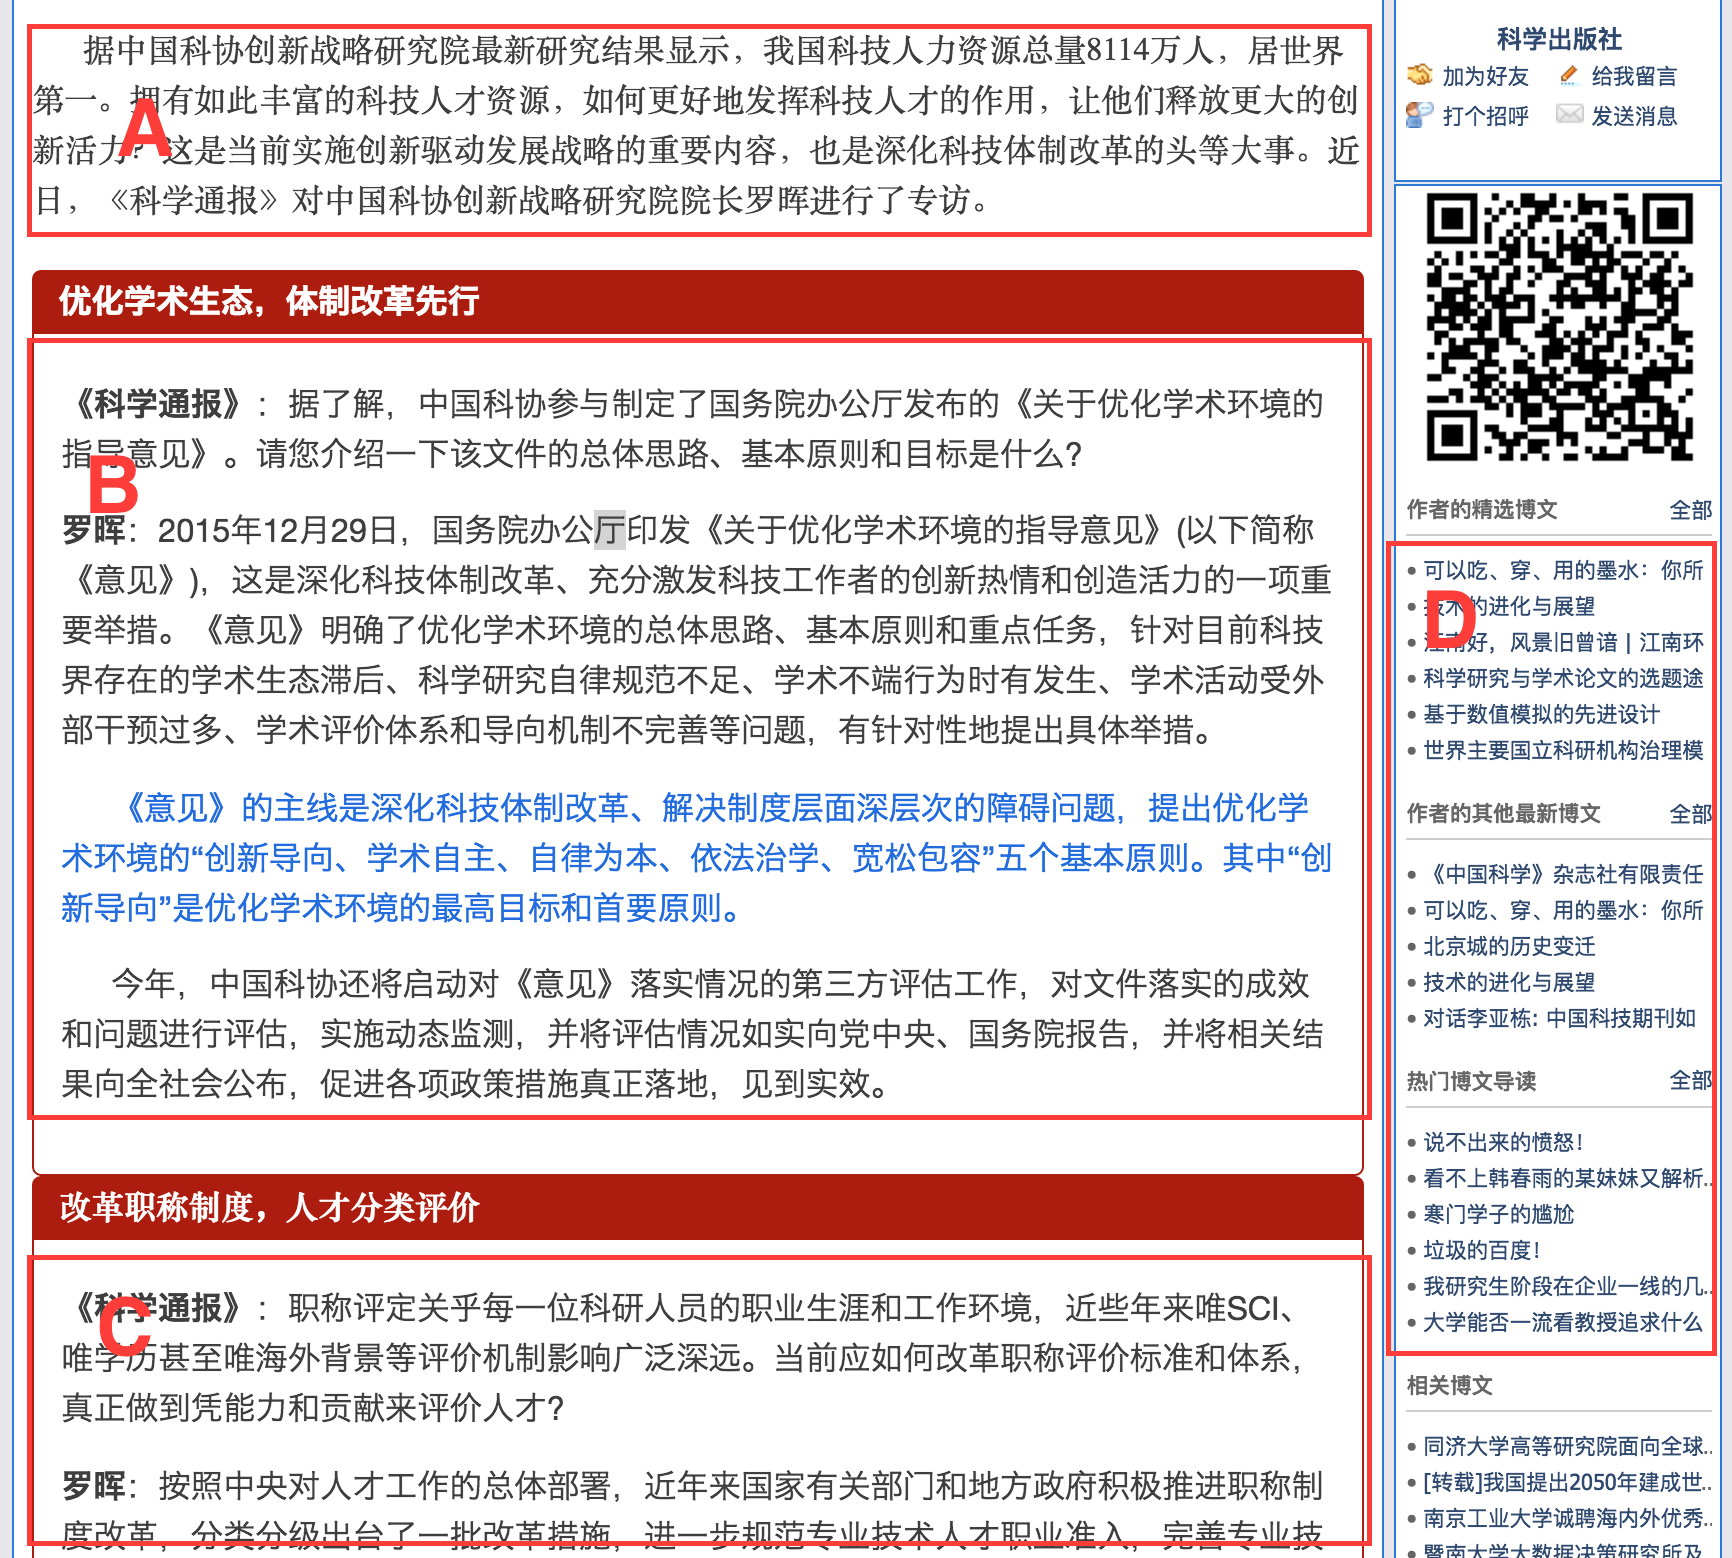
\includegraphics[width=0.9\textwidth,height=0.45\textheight]{blog-compare}
\caption{不同算法的抽取区域比较}
\label{fig:blog-compare}
\end{figure}

\section{本章小结}
\label{sec:cevc-conclusion}

本章研究针对新闻、博客的模板无关的自动化Web内容抽取技术,
首先简单介绍对比算法CETR(基于文本标签比)、CETD(基于文本密度)
和CEPR(基于文本标签路径比)的原理及实现细节,
然后提出一种基于有效字符的Web内容抽取算法CEVC。
该算法主要基于这样的观察,网页中不属于超链接并包含停止词的文本,更有可能是核心内容。
然后以一种自顶向下的方法,根据有效字符的分布,逐层在DOM树中确定核心内容区域。
最后在知名的中文新闻、博客网站上对四种方法进行了对比实验,
实验结果表明CEVC能达到平均95.8\%的F\textsubscript{1}-measure,
效果优于之前的算法CETR和CEPR。
虽然抽取性能和CETD相当,但在预处理阶段依赖更小,适用性更强。

%!TEX root = ../main.tex

\chapter{基于锚节点的论坛帖子抽取}

\section{概述}
随着互联网技术的快速发展,我们已经进入Web 2.0的时代\citeup{o2007web}。
不同于早期Web 1.0的网络应用,Web 2.0更强调用户生成内容(User-Generated Content,UGC),
可用性和互操作性,开始以用户为中心,体现资源平等的特点。
用户能够在社交网络中相互交流和协作,越来越多的人向虚拟社区贡献着自己产生的内容,
不同的观点和意见在这里交融碰撞,而不是在早期网站上那样被动地接收有限的内容。
网络论坛就是Web 2.0中的典型代表,用户可以在论坛上发帖、回帖进行讨论,
是一种交互性强、内容丰富而及时的网络应用。

一个典型的网络论坛组织结构如图~\ref{fig:forum-structure}~所示,
论坛一般按照话题分为若干个板块(Board);
板块内部用户围绕具体事件进行的一系列发帖、回帖统称为Thread,一般按照发帖时间线性排列;
在一个Thread内部,用户的每一次发帖是Post。
以网易论坛\footnote{http://bbs.163.com/}的一篇帖子为例,如图~\ref{fig:forum}~所示,
红色实线圈出的是每一个Post,它们按照时间顺序排列,
包含发帖人、发帖时间、发帖内容等元信息,共同组成了一篇帖子的核心内容。

\begin{figure}[htbp]
\centering
\begin{tikzpicture}[
sibling distance=5em,
every node/.style={rectangle,rounded corners,draw},
]
\node{Forum}
  child{node{Board A}
    child{node{Thread \#1}
      child{node{Post \#1}}
      child{node{Post \#2}}
      child{node{Post \#3}}
    }
    child{node{Thread \#2}}
  }
  child{node{Board B}}
  child{node{Board C}
    child{node{Thread \#1}}
    child{node{Thread \#2}}
  }
;
\end{tikzpicture}
\caption{论坛典型结构}
\label{fig:forum-structure}
\end{figure}

\begin{figure}[htbp]
\centering
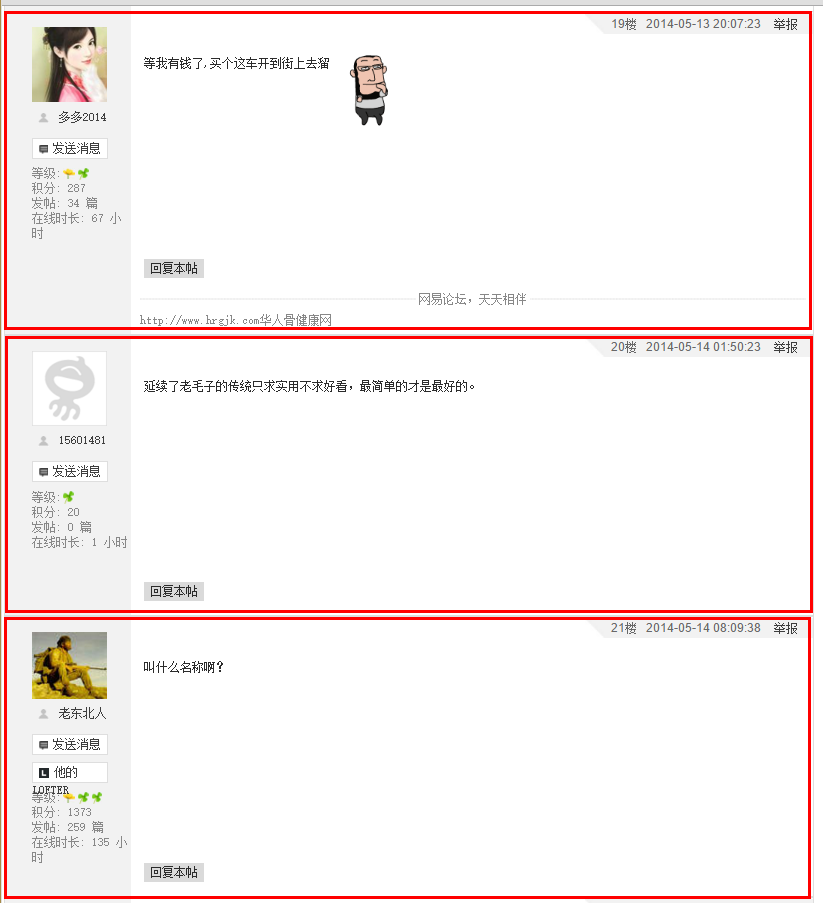
\includegraphics[width=0.9\textwidth,height=0.45\textheight]{forum}
\caption{论坛帖子实例}
\label{fig:forum}
\end{figure}

由于HTML网页所固有的半结构性,被设计为用户能够方便阅读,却不能被机器有效读取的形式。
虽然用户能够很容易区分不同的帖子,但面对结构样式各异的论坛网站,
如何从论坛网页中自动化地抽取帖子,转化为结构化的数据,
是一个很有挑战性的工作,也是舆情爬虫系统的重要环节。
本章利用论坛帖子中普遍存在的发帖时间信息作为锚节点,
提出一种基于锚节点的帖子抽取方法,~\ref{sec:pean-method}~节详述该方法
PEAN(Post Extraction via Anchor Nodes),
~\ref{sec:cevc-other}~节简单介绍对比算法MiBAT并给出算法实现细节,
~\ref{sec:pean-experiment}~节进行对比实验并分析结果。

\section{PEAN方法}
\label{sec:pean-method}

\subsection{树匹配算法}
\label{subsec:tree-match}

在数据记录抽取的研究工作中,很多方法\citeup{liu2003mining,song2010automatic}
都依赖树匹配算法来检测模板或衡量相似度,这里对树匹配问题给出形式化定义和简单介绍。

在~\ref{subsec:dom}~节中已经提到,网页可以解析为DOM树从而描述其结构信息。
树是广泛使用的数据结构,形式化称为有向无环图,
我们关心的DOM树是一种带标记的有序有根树(labeled ordered rooted tree)。
有序有根树意味着根节点固定,子节点之间的相对顺序也是固定的。

树由节点集合$V$和边集合$T$构成的二元组,$T=(V,E)$。
为了描述方便,记两个树$T_1$和$T_2$的节点集合分别为$V_1$和$V_2$。
在两个树的节点集合间寻找一个最优的一一映射,这就是树的比较或匹配。
树匹配\citeup{tai1979tree}的形式化定义如下:

\begin{definition}
\label{def:tree-mapping}
从$T_1$到$T_2$的匹配$M$,是一个有序二元组的集合$(u,v)$,$u \in V_1$,$v \in V_2$,
并对所有的$(u_1,v_1), (u_2,v_2) \in M$,满足以下条件:
\begin{enumerate}
\item $u_1 = u_2$,当且仅当$v_1 = v_2$;
\item $u_1$在$u_2$的左边,当且仅当$v_1$在$v_2$的左边;
\item $u_1$是$u_2$的祖先,当且仅当$v_1$是$v_2$的祖先。
\end{enumerate}
\end{definition}

在定义~\ref{def:tree-mapping}~中,
第一条保证了在一个匹配中每个节点最多出现一次,
第二条保证了节点间的兄弟关系在匹配中被保留,
第三条保证了节点间的父子关系在匹配中被保留。
直观上看,树匹配描述了把一个树转换为另一个树所需要的一系列操作,而忽略这些操作之间的顺序。
因此树匹配问题可以转化为树的编辑距离问题,找到最优的匹配就是找到代价最小的编辑操作。

树匹配问题的计算很消耗时间,解决它都需要平方复杂度以上的算法。
不过在具体的应用领域,可以使用一个受限制的树匹配描述,
自顶向下(top-down)匹配\citeup{selkow1977tree},
它在很多Web相关的研究中被成功运用。
其定义如下:

\begin{definition}
\label{def:top-down-mapping}
从$T_1$到$T_2$的匹配$M$如果满足以下条件就是自顶向下匹配:
对所有非根节点$u \in V_1$,$v \in V_2$,如果$(u,v) \in M$,
那么$(parent(u), parent(v)) \in M$,其中$parent(v)$是$v$的父节点。
\end{definition}

\begin{figure}[htbp]
\centering
\begin{tikzpicture}[
every node/.style={circle, draw},
level 1/.style={sibling distance=2cm},
level 2/.style={sibling distance=1cm},
gray/.style={circle, draw, fill=gray},
]
\node(A1){A}
  child{node(B1){B}}
  child{node(C1){C}
    child{node(D1){D}}
    child{node(E1){E}}
    child{node[gray]{F}}
  }
  child{node[gray]{G}
    child{node[gray]{I}}
  }
;
\node[right=5cm of A1](A2){A}
  child{node(B2){B}}
  child{node(C2){C}
    child{node(D2){D}}
    child{node(E2){E}}
  }
  child{node[gray]{H}
    child{node[gray]{I}}
    child{node[gray]{J}}
  }
;
\draw [dashed, thick, ->](A1) to [bend left](A2);
\draw [dashed, thick, ->](B1) to [bend left](B2);
\draw [dashed, thick, ->](C1) to [bend left](C2);
\draw [dashed, thick, ->](D1) to [bend left](D2);
\draw [dashed, thick, ->](E1) to [bend left](E2);
\end{tikzpicture}
\caption{自顶向下的树匹配}
\label{fig:top-down-mapping}
\end{figure}

如图~\ref{fig:top-down-mapping}~所示,
虚线所连接的就是这两个树之间的自顶向下匹配,灰色的节点是不能匹配的节点。
可以注意到,左树的G节点和右树的H节点处于同一位置,但由于标记不同而不匹配。
父节点不匹配后,虽然G节点和H节点都有相同的I节点,也不能匹配,这就是自顶向下限制的体现。

在自顶向下的限制之下,\cite{yang1991identifying}
给出了一个动态规划的树匹配算法,时间复杂度为$O(n^2)$。
如算法~\ref{algo:tree-match}~所示,
树匹配过程和通过动态规划求两个字符串的最长公共子序列有相似之处。
在两个根节点A和B匹配成功(标记相同)后,递归寻找A和B的第一级子树之间的最大匹配节点数,
构成一个$m \times n$的矩阵,$m$和$n$分别是A和B第一级子树的个数。
通过这个矩阵,使用动态规划的方法计算出A与B之间的最大匹配节点数。

\begin{algorithm}[htbp]
\caption{treeMatch(A, B)}
\label{algo:tree-match}
\KwIn{Tree $A$ and $B$}
\KwOut{Number of maximal matched nodes}

\If{the roots of $A$ and $B$ contain distinct labels}{
  \Return 0 \;
}
$m$ = the number of first-level subtrees of $A$ \;
$n$ = the number of first-level subtrees of $B$ \;
Initialize a $m \times n$ matrix $M$ with all zeros \;

\For{$i = 1$ \textbf{to} $m$}{
  \For{$j = 1$ \textbf{to} $n$}{
    $W[i,j]$ = treeMatch($A_i$, $B_j$) \;
    \tcc{$A_i$ and $B_j$ are the $i$th and $j$th first-level subtrees of 
    A and B respectively}
    $M[i,j]$ = max($M[i,j-1]$, $M[i-1,j]$, $M[i-1,j-1] + W[i,j]$) \;
  }
}
\Return $M[m,n] + 1$ \;
\end{algorithm}

\subsection{锚节点}
使用锚节点来辅助信息抽取,在\cite{song2010automatic}中就已经提出。
锚节点具有这样的特点:
\begin{itemize}
\item 作为关键的数据单元出现在每一个数据记录的结构化模板中;
\item 本身的文本具有一定的格式,容易抽取和识别。
\end{itemize}

发帖时间就是符合这样要求的一种锚节点。
首先论坛帖子中几乎都存在发帖时间,在图~\ref{fig:forum}~中,
3个不同帖子的楼层关系,正是靠发帖时间排序的。
其次发帖时间还是结构化模板中的一部分,格式固定,比如都位于帖子的右上角。
最后,形如“2014-05-13 20:07:23”这样的时间格式,使用简单的正则表达式就能有效识别。

图~\ref{fig:regex}~所示的就是本文使用的,用来识别发帖时间的正则表达式,
能够识别多种不同的时间格式:
\begin{itemize}
\item \texttt{2014-06-12 10:10:20}
\item \texttt{2014/06/12 10:10}
\item \texttt{2014/6/12 10:10:20}
\end{itemize}

\begin{figure}[htbp]
\centering
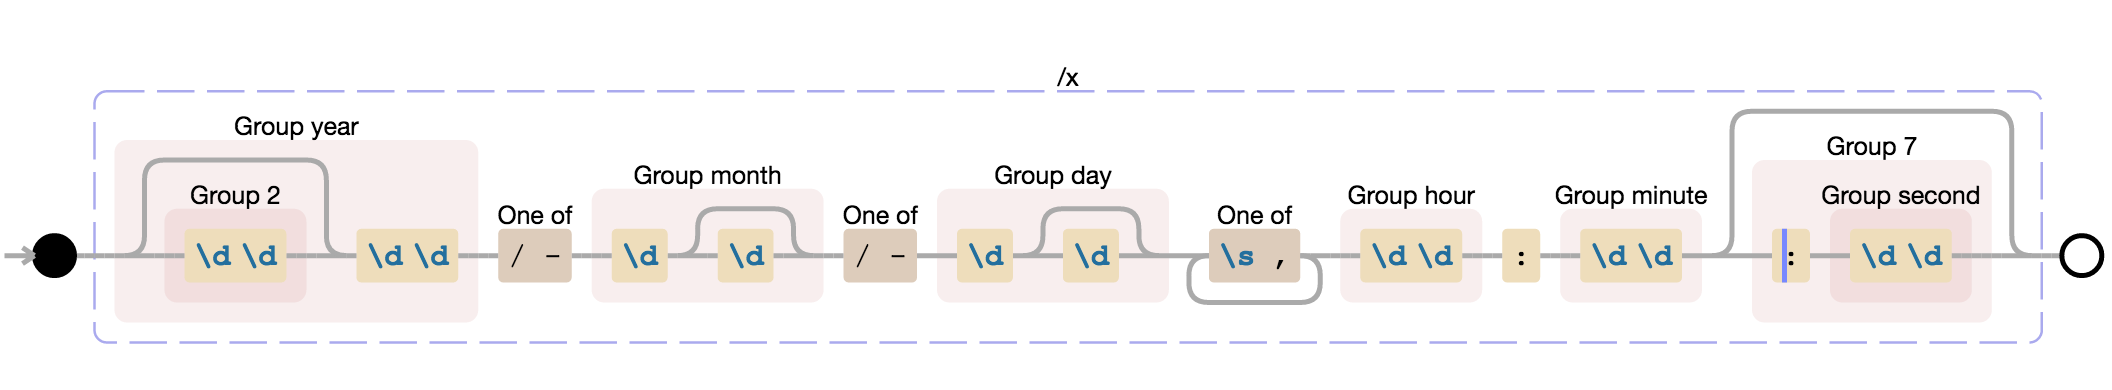
\includegraphics[width=1.0\textwidth]{regex}
\caption{识别发帖时间的正则表达式}
\label{fig:regex}
\end{figure}

如果以发帖时间作为锚节点(Pivot),那么在DOM树中包含发帖时间的最底层的节点,
就定义为锚节点:

\begin{definition}
\label{def:pivot}
$i$是DOM中的一个节点,如果$\vert D_i \vert > 0$且
$\forall j \in descendant(i)$都有$\vert D_j \vert = 0$,
那么$i$就是锚节点
\end{definition}

定义~\ref{def:pivot}~中,$\vert D_i \vert$表示节点$i$的文本中发帖时间的个数,
$descendant(i)$表示$i$的子孙节点集合。

我们可以计算出当前节点所包含的锚节点个数Pivots,
通过Pivots来指导程序发现帖子存在的区域。
类似于算法~\ref{algo:cevc-count}~,这是一个自顶向下的递归计算过程,
Pivots被作为属性,存储在相应节点中。
同样在处理之前,需要从DOM树中移除
\texttt{<script>},\texttt{<style>}和\texttt{comment}。
经过算法countPivots处理之后,我们可以得到一个标注了各个节点Pivots的HTML页面,
如图~\ref{fig:forum-stepinto}~所示。

\begin{figure}[htbp]
\centering
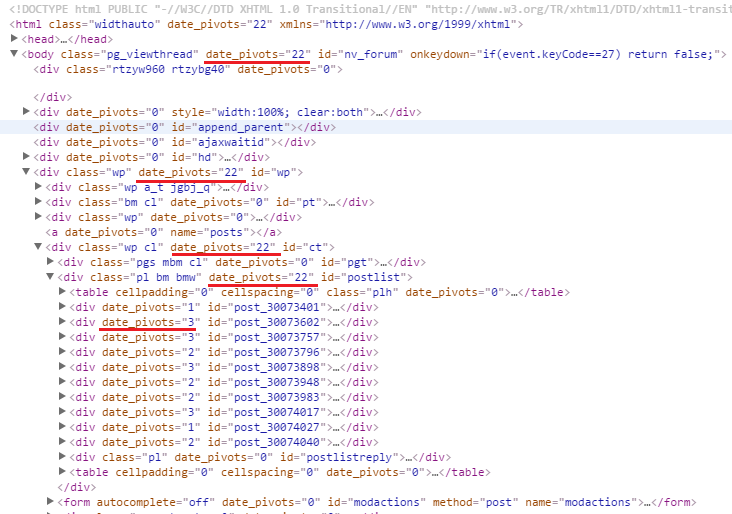
\includegraphics[width=0.9\textwidth]{forum-stepinto}
\caption{时间锚节点示例}
\label{fig:forum-stepinto}
\end{figure}

\subsection{定位帖子节点}
经过大量实例分析,我们发现论坛帖子有一个共同的特点,它们都位于DOM树中同一个父节点之下。
图~\ref{fig:forum-stepinto}~的帖子形式如\texttt{<div\#post\_30073401>},
都位于父节点\texttt{<div\#postlist>}之下。
因为帖子之间是相似的,它们在逻辑地位上是平等的,
论坛网站的服务端程序从数据库中取出数据记录,经过前端模板的渲染最终形成网页,
为了统一对它们进行调整和控制,隶属于同一个父节点是很自然的。

从图~\ref{fig:forum-stepinto}~中可以看到,每个帖子都至少包含一个时间锚节点,
直观地看,时间锚节点密集的区域就是帖子存在的区域。
如果从\texttt{<body>}节点开始,每次都选择时间锚节点最多的子节点深入,
就能定位出一条从\texttt{<body>}通往帖子节点的正确路径,
如图~\ref{fig:forum-stepinto}~中红线标示的节点。
为了描述方便,将这条路径在例~\ref{ex:rmd-mpr}~中列出,其中RMD和MPR在下文中详述。

\begin{figure}[htbp]
\begin{example}
\label{ex:rmd-mpr}
RMD和MPR计算过程
\end{example}
\begin{verbatim}
1. <body> Pivots=22 RMD=0 MPR=1
2. <div#wp> Pivots=22 RMD=0 MPR=1
3. <div#ct> Pivots=22 RMD=0 MPR=1
4. <div#postlist> Pivots=22 RMD=0.29 MPR=0.14 帖子的父节点
5. <div#post_30073602> Pivots=3 RMD=0 MPR=1
6. ...
\end{verbatim}
\end{figure}

每次沿着Pivots最大的子节点不断深入,这个过程不能一直持续下去,
否则会陷入叶节点中,而错失最终的目标节点。
我们定义两个指标,来判断何时停止向下深入的过程。

\begin{definition}
\label{def:rmd}
相对平均偏差(Relative Mean Deviation,RMD)是样本的平均偏差除以样本均值的绝对值:
\begin{equation}
RMD = \frac{\frac{1}{n} \sum_{i=1}^{n} \vert x_i - \bar x \vert}
{\vert \bar x \vert}
\end{equation}
\end{definition}

把同一个父节点下的子节点的时间锚节点个数组成一组样本,去除那些锚节点数为零的样本,
然后计算相对平均偏差RMD,来衡量锚节点在子节点中分布的均匀程度。

因为锚节点属于格式化模板中的一部分,在帖子中分布是较为均匀的,
所以当RMD小于某个阈值时,表明锚节点分布均匀,当前节点下很可能包含一组帖子。
当父节点只有一个子节点包含锚节点时,相对平均偏差为零,这种特殊情况下毫无疑问应当继续深入。
在例~\ref{ex:rmd-mpr}~中,1-3行的RMD都为零,时间锚节点高度集中在一个子节点中。

\begin{definition}
\label{def:mpr}
$i$是DOM树中的一个节点,$i$的最大子节点锚节点占比MPR(Max Pivots Ratio)如下所示,
其中$P_i$表示$i$的锚节点个数,$j$是$i$的子节点:
\begin{equation}
MPR_i = max_{j \in children(i)} \frac{P_j}{P_i}
\end{equation}
\end{definition}

在DOM树中每次向下深入一步,我们认为最大子节点包含了父节点的绝大部分锚节点。
当定义~\ref{def:mpr}~中的MPR低于一个阈值时,
表明最大子节点的锚节点并不足以在父节点中占据统治地位,继续向下深入可能会损失信息。

通过RMD和MPR联合确定停止向下深入的条件,即RMD和MPR都小于各自的阈值时,
向下深入的过程立即终止,当前节点被标记为帖子的父节点。
此时,extract过程负责从当前节点的子节点中筛选出真正的帖子。
这个过程详见算法~\ref{algo:pean-stepinto}~。

第~\ref{algo:line:rmd}~行,
在比较RMD和MPR时,还需要确定pivots集合的大小,即包含锚节点的子节点不能只有一个。
在这种情况下单一样本的RMD一定为零,却并不意味着子节点中锚节点分布均匀,
而是锚节点全部集中在一个子节点中,必须继续向下深入。

算法~\ref{algo:pean-stepinto}~能够很快运行结束,因为它至多被递归调用$h$次,
$h$是DOM树的深度,时间复杂度为$O(h)$。

\begin{algorithm}[htbp]
\caption{stepInto(N)}
\label{algo:pean-stepinto}
\KwIn{DOM node N}
\KwOut{Posts}

pivots = $\emptyset$ \;
maxNode = null \;
\For{$C \in N.children()$}{
  \If{$C.pivots > max(pivots)$}{
    maxNode = C \;
  }
  pivots.append(C.pivots) \;
}

\If{maxNode is not null}{
  RMD = computeRMD(pivots) \;
  MPR = max(pivots) / sum(pivots) \;
  \eIf{$pivots.length > 1$ \textbf{and} $RMD < \alpha$ 
    \textbf{and} $MPR < \beta$}{ \label{algo:line:rmd}
    \Return extract(N) \;
  }{
    stepInto(maxNode) \;
  }
}
\end{algorithm}

\subsection{筛选候选帖子}
在定位了帖子的父节点后,筛选真正的帖子并不是一件简单的工作,
因为帖子的兄弟节点中可能包含很多噪声部分,例如广告、装饰性内容等。
以一篇西陆论坛\footnote{http://club.xilu.com/}的帖子为例,
如图~\ref{fig:forum-noise}~所示,红色实线标示的是真正的帖子,
第一个为楼主发布的主帖,剩下10个为回帖。

这些帖子都位于父节点\texttt{<body>}之下,但\texttt{<body>}之下还有很多非帖子的节点,
\texttt{<div\#BAIDU\_UNION>}是百度联盟提供的广告,
\texttt{<div\#d\_main>}是主帖前后的推荐信息。
如何准确筛选真正的帖子,需要利用帖子和帖子之间DOM树结构的相似性。

\begin{figure}[htbp]
\centering
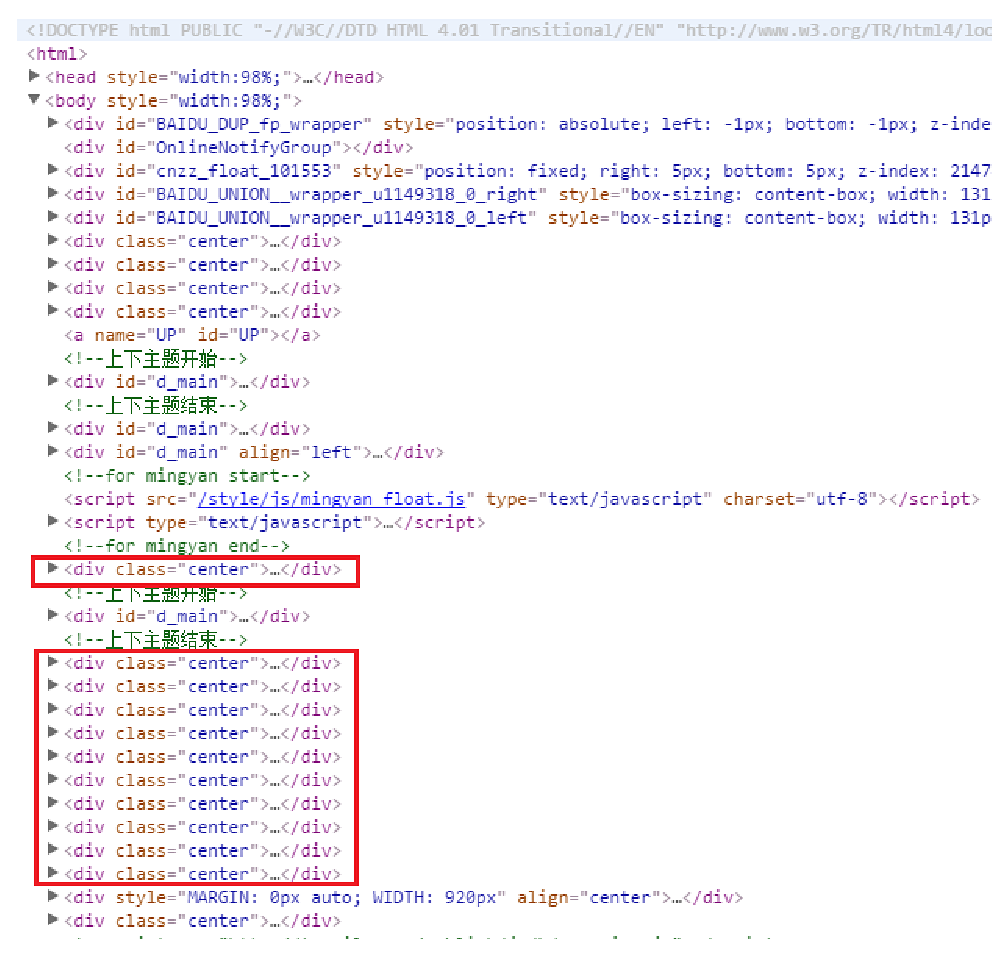
\includegraphics[width=0.9\textwidth]{forum-noise.eps}
\caption{帖子中的噪声}
\label{fig:forum-noise}
\end{figure}

在~\ref{subsec:tree-match}~节的树匹配算法的基础上,可以给出树的相似度定义。

\begin{definition}
\label{def:tree-sim}
已知$M$是两个树$T_1$和$T_2$的匹配,则$T_1$和$T_2$的相似度是:
\begin{equation}
TreeSim(T_1, T_2) = \frac{\vert M \vert}
{(\vert V_1 \vert + \vert V_2 \vert) / 2}
\end{equation}
\end{definition}

其中$\vert M \vert$是$M$中匹配节点的对数,
$\vert V_1 \vert$和$\vert V_2 \vert$分别是$T_1$和$T_2$节点的个数。
从定义~\ref{def:tree-sim}~中可知,树的相似度受树节点规模的影响,
在$\vert M \vert$相同的情况下,
如果$\vert V_1 \vert$或$\vert V_2 \vert$增大就会稀释整个相似度。

我们从图~\ref{fig:post-match}~中的例子分析,
这两个子树代表两个帖子,虚线连接的是相互匹配的节点。
帖子第一层子节点中,代表发帖时间和发帖内容的节点都能够相互匹配,
但灰色节点标志的用户生成内容却不能匹配。
论坛帖子有别于商品展示信息,它的内容由用户生成(UGC),
具有很高的自由度,因此体现出高度差异化和多样性。
左边帖子直接包含文本和换行标签\texttt{<br>},
右边帖子则通过\texttt{<p>}包裹文本,并提供了一张图片\texttt{<img>}。

\begin{figure}[htbp]
\centering
\begin{tikzpicture}[
level 1/.style={sibling distance=2cm},
level 2/.style={sibling distance=2cm},
level 3/.style={sibling distance=1cm},
tag/.style={circle, draw},
leaf/.style={rectangle, draw, text width=2cm},
gray/.style={fill=gray},
]
\node[tag](A1){div}
  child{node[tag](B1){div}
    child{node[leaf]{2016-02-16}}
  }
  child{node[tag](C1){div}}
  child{node[tag](D1){div}
    child{node[leaf, gray]{There is something}}
    child{node[tag, gray]{br}}
  }
;
\node[tag, right=8cm of A1](A2){div}
  child{node[tag](B2){div}
    child{node[leaf]{2016-03-10}}
  }
  child{node[tag](C2){div}}
  child{node[tag](D2){div}
    child{node[tag, gray]{p}
      child{node[leaf, gray]{The photo is amazing!}}
    }
    child{node[tag, gray]{img}}
  }
;
\draw [dashed, thick, ->](A1) to [bend left](A2);
\draw [dashed, thick, ->](B1) to [bend left](B2);
\draw [dashed, thick, ->](C1) to [bend left](C2);
\draw [dashed, thick, ->](D1) to [bend left](D2);
\end{tikzpicture}
\caption{帖子的匹配}
\label{fig:post-match}
\end{figure}

如果直接使用定义~\ref{def:tree-sim}~的树相似度计算,
就会被高度自由的UGC节点干扰,使两个帖子原本应该很高的相似度降低,最后被认为不相似而遗漏。
和字符串的最长公共子序列类似,最大匹配节点数反映了两个树之间“重合”部分的大小。
虽然UGC内容带来的结构、形式差异会导致帖子间相似度参差不齐,
但相互之间能够匹配的最大节点数却比较稳定,可以利用这个“重合”部分来度量相似性。

从候选子节点中筛选真正帖子的过程extract,如算法~\ref{algo:pean-extract}~所示。
算法~\ref{algo:pean-stepinto}~中选定的maxNode在这里被当做基准节点,
其它至少包含一个锚节点的兄弟节点一一与之进行树匹配计算,
然后以节点作为key、最大匹配节点数作为value存储在一个map数据结构中。

基准节点maxNode被认定为帖子,output过程将其内容输出。
其它节点按照和基准节点之间重合部分的大小,从高到低排列,
虽然它们彼此的相似度可能参差不齐,但重合度却比较稳定。
按照这个顺序遍历最大匹配节点个数,如果发现某个最大匹配节点数低于前者的一半,
就认为筛选结束,该节点之前的都属于目标帖子,而放弃之后重合度太低的节点。

\begin{algorithm}[htbp]
\caption{extract(N, maxNode)}
\label{algo:pean-extract}
\KwIn{DOM node N, maxNode}
\KwOut{Posts}

mappings = $\emptyset$ \;
\For{$C \in N.children()$}{
  \If{$C \neq maxNode$ \textbf{and} $C.pivots > 0$}{
    mappings[C] = treeMatch(C, maxNode) \;
  }
}

output(maxNode) \;
lastNum = 0 \;
\For{$C \in$ mappings ordered from high to low}{
  \If{$mappings[C] < lastNum / 2$}{
    \textbf{break} \;
  }
  lastNum = mappings[C] \;
  output(C) \;
}
\end{algorithm}

记候选帖子数量为$m$,每个帖子的平均节点数为$n$。
算法~\ref{algo:pean-extract}~的运算分为两部分:
\begin{enumerate}
\item 首先是基准节点和候选帖子节点之间的树匹配过程,
因为treeMatch的复杂度为$O(n^2)$,所以其复杂度为$O(mn^2)$。
\item 另一部分是对候选帖子的排序、遍历过程,
排序复杂度为$O(m\log m)$,所以其复杂度为$O(m\log m)$。
\end{enumerate}

一般情况下,由于论坛结构和UGC内容日趋丰富,再加上分页对单篇网页帖子数量的限制,
候选帖子数量$m$小于帖子的平均节点数$n$,自然有$n^2 > \log m$,
算法~\ref{algo:pean-extract}~extract的总体时间复杂度为$O(mn^2)$。

\subsection{算法实现}
本文中PEAN算法使用Python 2.7实现。

\section{对比算法及实现}
\label{sec:pean-other}

本章的对比算法为MiBAT\citeup{song2010automatic}
(\textbf{Mi}ning data records 
\textbf{B}ased on \textbf{A}nchor \textbf{T}rees),
该算法也通过Python 2.7实现。

面对论坛帖子中UGC内容格式自由、复杂多变而干扰相似度计算的问题
(图~\ref{fig:post-match}~),MiBAT的主要解决方法是,
在树相似度计算过程中,尽可能选择隶属于格式化模板的一部分节点进行比较,
而不是将所有节点全部考虑进去。
这里相互比较的节点子集,称为tree fragments。
树相似度定义扩展为:

\begin{definition}
\label{def:tree-ex-sim}
已知$M$是两个树$T_1$和$T_2$的匹配,$f$是tree fragment选择函数,
则$T_1$和$T_2$在$f$作用下的相似度是:
\begin{equation}
TreeSim_f(T_1, T_2) = \frac{M \cap (f(V_1) \times f(V_2))}
{(\vert f(V_1) \vert + \vert f(V_2) \vert) / 2}
\end{equation}
\end{definition}

定义~\ref{def:tree-ex-sim}~中,
$f(V_1) \times f(V_2) = {(u,v) \vert u \in f(V_1), v \in f(V_2)}$。
最佳情况是,tree fragment选择函数直接选取了树的模板部分,但这难以做到。
\cite{song2010automatic}定义了几种tree fragment选择函数,
并最终使用了Pivot and Siblings(PS)选择函数。
简单来说,就是用锚节点和锚节点的兄弟节点作为模板部分的近似,
从而规避UGC节点对相似度计算的干扰。

\section{实验与分析}
\label{sec:pean-experiment}

\subsection{评价指标}
为了验证算法的抽取效果,我们定义标准评价指标准确率Precision、召回率Recall和
F\textsubscript{1}。
通过比较算法抽取的帖子集合$e$和金标准的帖子集合$g$,Precision、Recall和
F\textsubscript{1}可以如下计算:

\begin{equation}
P = \frac{e \cap g}{\vert e \vert}, R = \frac{e \cap g}{\vert g \vert}
\end{equation}
\begin{equation}
F_1 = \frac{2 \times P \times R}{P + R}
\end{equation}

\subsection{数据集}
为了验证帖子抽取算法在实际中文论坛上的抽取效果,
我们从知名的网址导航网站hao123\footnote{https://www.hao123.com/}
和360导航\footnote{https://hao.360.cn/}
中任意选取了20个知名的论坛网站作为测试对象,如表~\ref{tbl:forum-dataset}~所示。
从采集的网页中,去除失效的、没有回帖的网页,
总计有效网页973个,平均每个网站50个以内。

\begin{table}[htbp]
\caption{论坛数据集}
\label{tbl:forum-dataset}
\vspace{0.5em}\centering\wuhao
\begin{tabular}{llll}
\toprule[1.5pt]
编号 & 论坛名称 & 论坛代码 & 网址 \\
\midrule[1pt]
1 & 网易论坛 & 163 & http://bbs.163.com/ \\
2 & 360安全社区 & 360safe & http://bbs.360safe.com/ \\
3 & 55BBS论坛 & 55bbs & http://bbs.55bbs.com/ \\
4 & 腾讯论坛 & qq & http://bbs.ent.qq.com/ \\
5 & 环球论坛 & huanqiu & http://bbs.huanqiu.com/ \\
6 & 春秋社区 & ichunqiu & http://bbs.ichunqiu.com/ \\
7 & 卡饭论坛 & kafan & http://bbs.kafan.cn/ \\
8 & 远景论坛 & pcbeta & http://bbs.pcbeta.com/ \\
9 & 看雪学院 & pediy & http://bbs.pediy.com/ \\
10 & 瑞丽论坛 & rayli & http://bbs.rayli.com.cn/ \\
11 & 天涯社区 & tianya & http://bbs.tianya.cn/ \\
12 & 铁血论坛 & tiexue & http://bbs.tiexue.net/ \\
13 & 精睿 & vc52 & http://bbs.vc52.cn/ \\
14 & 华声论坛 & voc & http://bbs.voc.com.cn/ \\
15 & 中华网论坛 & china & http://club.china.com/ \\
16 & 新浪论坛 & sina & http://club.history.sina.com.cn/ \\
17 & 凯迪社区 & kdnet & http://club.kdnet.net/ \\
18 & 宽带山 & pchome & http://club.pchome.net/ \\
19 & 西陆论坛 & xilu & http://club.xilu.com/ \\
20 & 泡泡俱乐部 & pcpop & http://pop.pcpop.com/ \\
\bottomrule[1.5pt]
\end{tabular}
\end{table}

数据的采集和标注都需要消耗很多的精力,为了节省人力成本,
我们通过构建特定论坛的包装器来解决这个问题。
如例~\ref{ex:forum-wrapper}~所示,
FORUM是Python的字典结构,以key-value对的形式存储各个论坛的详细配置。

\begin{figure}[htbp]
\begin{example}
\label{ex:forum-wrapper}
论坛包装器示例
\end{example}
\begin{verbatim}
FORUM = {
  '163': {
    'name': '网易论坛',                   # 论坛名称
    'home': 'http://bbs.163.com/',        # 论坛主页地址
    'board': 'http://bbs.news.163.com/',  # 论坛板块地址
    'thread': ['ul.rankList a[href]'],    # 论坛thread的CSS选择符 
    'post': ['div.tie-item'],             # 论坛帖子的CSS选择符
  },
}
\end{verbatim}
\end{figure}

以网易论坛为例,采集程序从板块地址\url{http://bbs.news.163.com/}入手,
得到某个板块的网页,然后通过thread的CSS选择符定位每个thread的url。
选择符\texttt{ul.rankList a[href]}的含义是,
选择所有\texttt{<ul class='rankList'>}标签下的,
有\texttt{href}属性的\texttt{<a>}标签。
同理,通过帖子的CSS选择符可以标注真正的帖子,供后续实验分析。

这里的CSS选择符可以是一个列表,包含不止一个选择符,以应对更负责的情况。
例如在凯迪社区的配置中,帖子既可能是\texttt{div.reply-box},
也可能是\texttt{div.posted-box-add},对应主帖和后续跟帖。

\subsection{实验结果}

\subsection{结果分析}


% 参考文献
\defaultfont
\bibliographystyle{GBT7714-2005}
\addcontentsline{toc}{chapter}{参考文献}
\addtolength{\bibsep}{-0.8em}
\nocite{*}
\bibliography{reference}

% 附录
\chapter*{攻读硕士学位期间发表的论文及其他成果}
\phantomsection
\addcontentsline{toc}{chapter}{攻读硕士学位期间发表的论文及其他成果}

\noindent\textbf{(一)发表的学术论文}
\begin{publist}
\item	\underline{XXX},XXX. Static Oxidation Model of Al-Mg/C Dissipation Thermal Protection Materials[J]. Rare Metal Materials and Engineering, 2010, 39(Suppl. 1): 520-524.(SCI~收录,IDS号为~669JS,IF=0.16)
\item XXX,\underline{XXX}. 精密超声振动切削单晶铜的计算机仿真研究[J]. 系统仿真学报,2007,19(4):738-741,753.(EI~收录号:20071310514841)
\item XXX,XXX. 局部多孔质气体静压轴向轴承静态特性的数值求解[J]. 摩擦学学报,2007(1):68-72.(EI~收录号:20071510544816)
\item XXX,XXX. 硬脆光学晶体材料超精密切削理论研究综述[J]. 机械工程学报,2003,39(8):15-22.(EI~收录号:2004088028875)
\item XXX,XXX. 基于遗传算法的超精密切削加工表面粗糙度预测模型的参数辨识以及切削参数优化[J]. 机械工程学报,2005,41(11):158-162.(EI~收录号:2006039650087)
\item XXX,XXX. Discrete Sliding Mode Cintrok with Fuzzy Adaptive Reaching Law on 6-PEES Parallel Robot[C]. Intelligent System Design and Applications, Jinan, 2006: 649-652.(EI~收录号:20073210746529)
\end{publist}

\chapter*{哈尔滨工业大学学位论文原创性声明和使用权限}
\phantomsection
\addcontentsline{toc}{chapter}{哈尔滨工业大学学位论文原创性声明和使用权限}

\vspace{\baselineskip}
\begin{center}{\xiaosan \heiti 学位论文原创性声明}\end{center}
\vspace{1em}

本人郑重声明:此处所提交的学位论文《\ctitle》,是本人在导师指导下,在哈尔滨工业大学攻读学位期间独立进行研究工作所取得的成果,且学位论文中除已标注引用文献的部分外不包含他人完成或已发表的研究成果。对本学位论文的研究工作做出重要贡献的个人和集体,均已在文中以明确方式注明。

\vspace{\baselineskip}
\hspace{6em}作者签名:\hfill 日期:\hspace{2.5em}年\hspace{1.5em}月\hspace{1.5em}日

\vspace{2\baselineskip}
\begin{center}{\xiaosan \heiti 学位论文使用权限}\end{center}
\vspace{1em}

学位论文是研究生在哈尔滨工业大学攻读学位期间完成的成果,知识产权归属哈尔滨工业大学。学位论文的使用权限如下:

(1)学校可以采用影印、缩印或其他复制手段保存研究生上交的学位论文,并向国家图书馆报送学位论文;(2)学校可以将学位论文部分或全部内容编入有关数据库进行检索和提供相应阅览服务;(3)研究生毕业后发表与此学位论文研究成果相关的学术论文和其他成果时,应征得导师同意,且第一署名单位为哈尔滨工业大学。

保密论文在保密期内遵守有关保密规定,解密后适用于此使用权限规定。

本人知悉学位论文的使用权限,并将遵守有关规定。


\vspace{2\baselineskip}
\hspace{6em}作者签名:\hfill 日期:\hspace{2.5em}年\hspace{1.5em}月\hspace{1.5em}日

\vspace{2\baselineskip}
\hspace{6em}导师签名:\hfill 日期:\hspace{2.5em}年\hspace{1.5em}月\hspace{1.5em}日

\chapter*{致\quad 谢}
\phantomsection
\addcontentsline{toc}{chapter}{致谢}

在哈工大计算机学院度过的三年硕士研究生生活中,我得到了许多无私的帮助,
也感受了网安实验室家一般的温暖。
值此论文完成之际,向所有关心、支持和帮助我的老师、同学和亲人们致以衷心感谢。

首先衷心感谢我的导师张宏莉教授。
张老师严谨认真的治学态度,高屋建瓴的学术视角,平易近人的为人风格让我受益匪浅,
从毕业论文的选题到研究工作中的困难,从实验室的项目到未来的工作,
张老师都给我宝贵的建议和指导,让我收获了知识和能力,更得到了难得的锻炼。

感谢余翔湛老师几年来对我的耐心指导和帮助。
余老师为人宽厚谦和,对我的每次请教都耐心细致地讲解,
无论是学习中的问题还是工作中的问题,都给了我很多帮助。
余老师渊博的知识、严谨的作风、科学的态度深深地感染和激励着我,让我受益良多。

感谢叶麟师兄、王星师兄,你们在实验室的工程项目上给予我很多指导,
作为实验室的青年教师,你们勇于承担责任、勤勤恳恳兢兢业业的作风潜移默化地影响了我,
怀念与你们共同奋斗的日日夜夜!

感谢实验室的张伟哲老师、何慧老师、翟健宏老师、张宇老师、张羽老师、张玥老师等,
是这些老师们的专业素养营造了实验室良好的学术研究氛围。
感谢实验室的秘书左冬梅老师、赵老师,
你们处处为学生着想,为实验室营造了舒适的学习工作环境。

感谢牛林华、商兴奇、吴钧超、尹志敏师兄,
感谢夏重达、王岳、徐洋、王松、李肖强、赵尚杰、谢虎成、孟媛媛以及实验室的其他同学,
感谢李英俊、詹东阳、丛小亮、赵卫晨、姚崇崇、韩硕、何泽宇、淼爷、宋、叁姐、云超和其他师弟师妹们,
是你们的陪伴让我度过了充满回忆的硕士生涯。

感谢主席、泽神、晓亮、大镕哥,认识你们是我人生的宝贵财富,
也祝愿你们早日毕业、前程似锦!

最后感谢我的父母,是你们的辛勤付出让我在近二十载的求学生涯中能够全力以赴,
今天的成果离不开你们的鼓励与支持!
还要感谢我的姐姐,家庭永远是我最坚实的后盾!


\clearpage

\end{document} 
